\newpage
\section{細径MPAを用いた歩脚ロボットの開発}
本章では実際に作製した歩脚ロボットの構成について述べる.
まず初めに羽状配置での動作確認を行うために作製した予備実験の機体の構成とその実験結果についてまとめ,その次に実際のズワイガニの構成と寸法をもとにした機体とその動作実験の結果について述べる.
%%%%%%%%%%%%%%%%%%%%%%%%%%%%%%%%%%%%%%%%%%%%%%%%%%%%%%%%%
\begin{figure}[b]
  \centering
  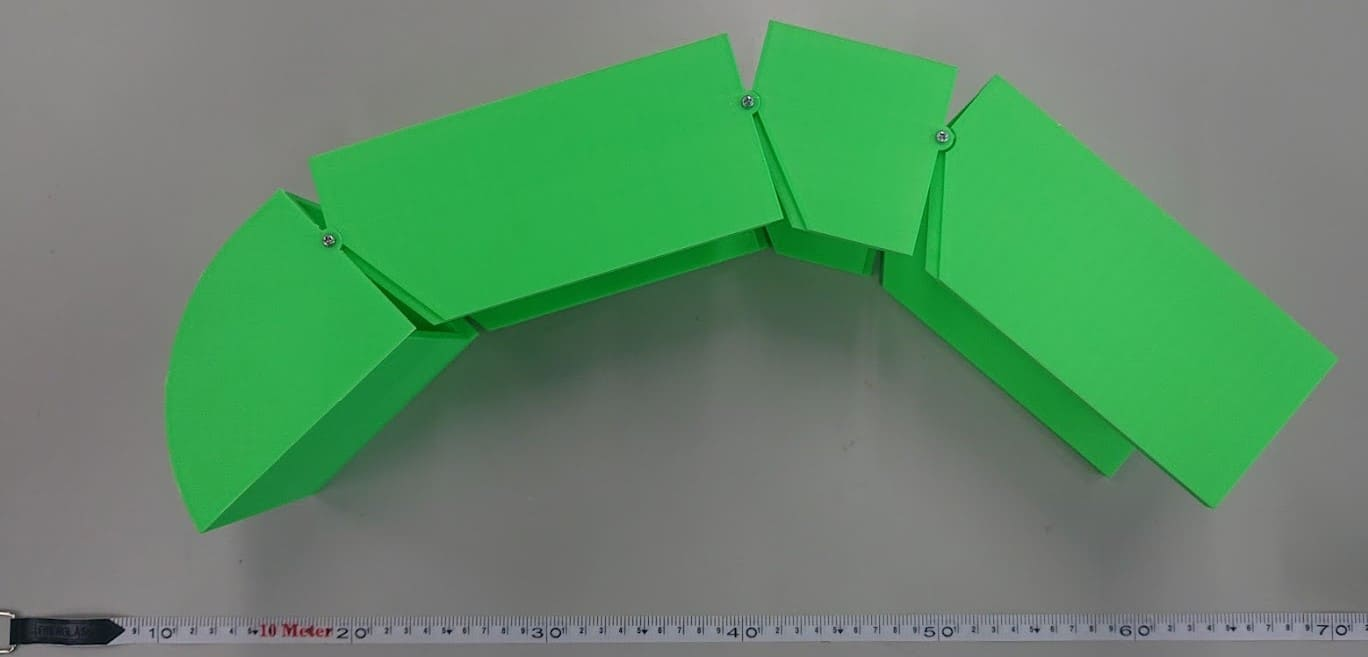
\includegraphics[scale=0.21]{image/greenkitai.JPG}
  \caption{実験機の外観}
  \label{fig:pkitai}
\end{figure}
%
\begin{figure}[t]
  %
  \begin{minipage}{0.5\hsize}
    \centering  
    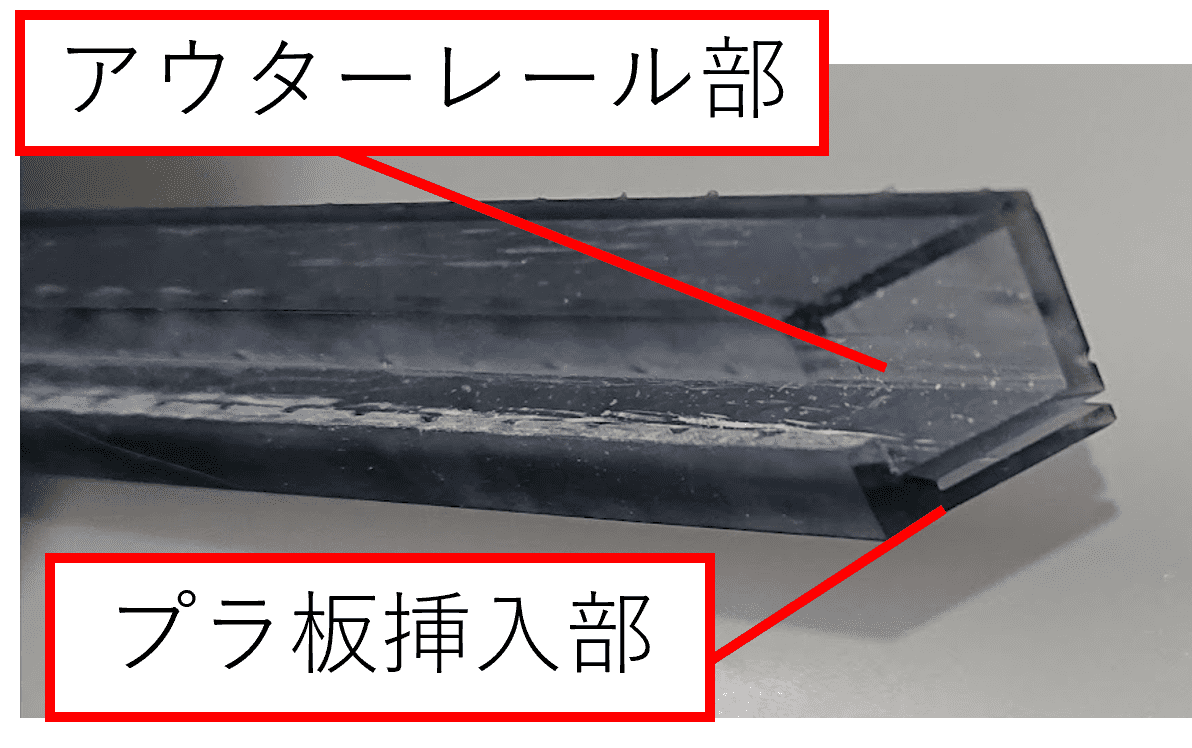
\includegraphics[scale=0.16]{image/syuseki_yobi.png}
    \subcaption{腱部分}
    \label{fig:pken}
  \end{minipage}
  \begin{minipage}{0.5\hsize}
    \centering
    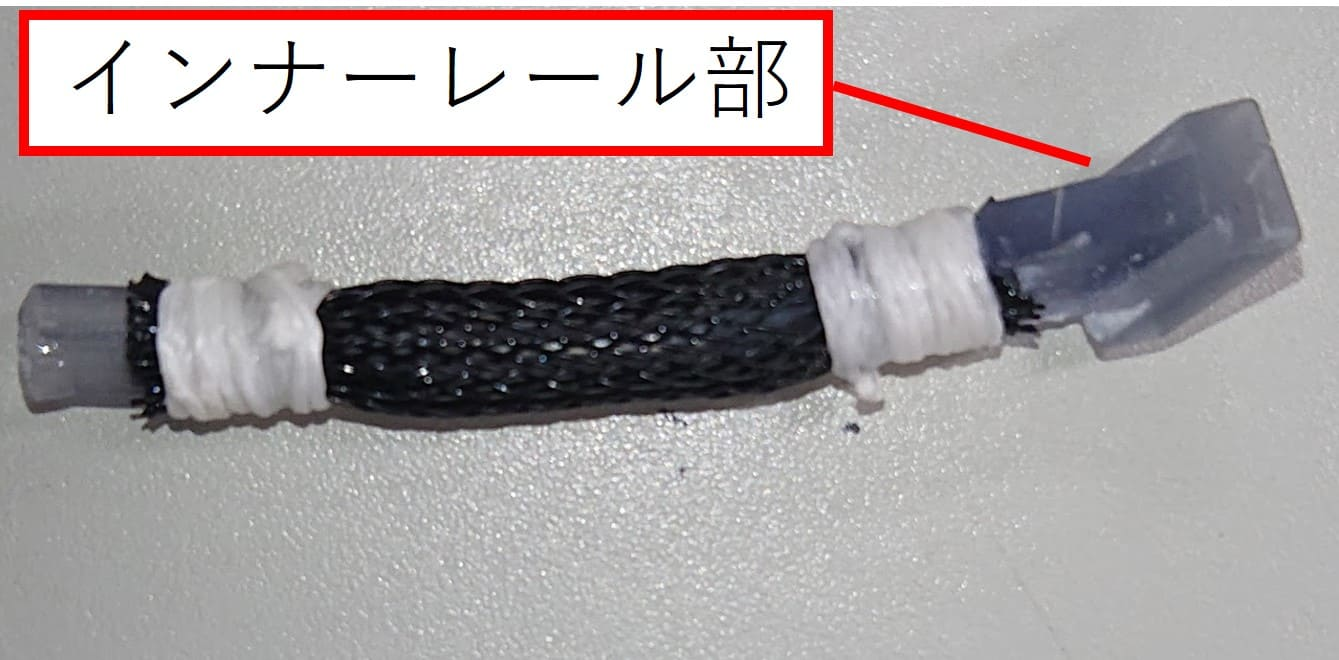
\includegraphics[scale=0.16]{image/syuseki_yobi2.jpg}
    \subcaption{MPA端部}
    \label{fig:ptanbu}
  \end{minipage}\\

  \begin{minipage}{0.5\hsize}
    \centering
    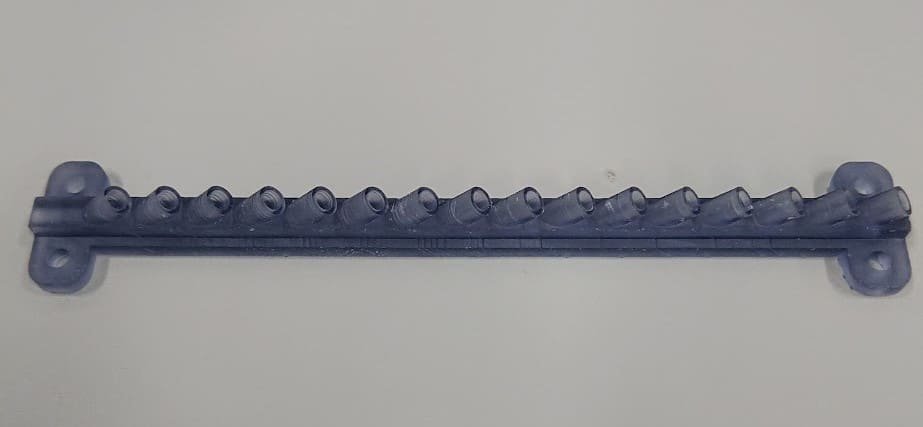
\includegraphics[scale=0.22]{image/airtube_yobi.jpg}
    \subcaption{空気分岐部品}
    \label{fig:pairtube}
  \end{minipage}
  \begin{minipage}{0.5\hsize}
    % \vspace{3mm}
    \centering  
    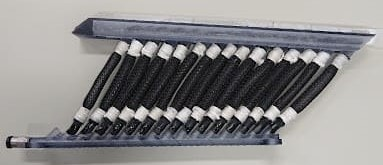
\includegraphics[scale=0.75]{image/yobi_syuseki.JPG}
    \subcaption{半羽状筋状に集積した様子}
    \label{fig:psyuseki}
  \end{minipage}\\

  \begin{minipage}{1\hsize}
    \vspace{3mm}
    \centering
    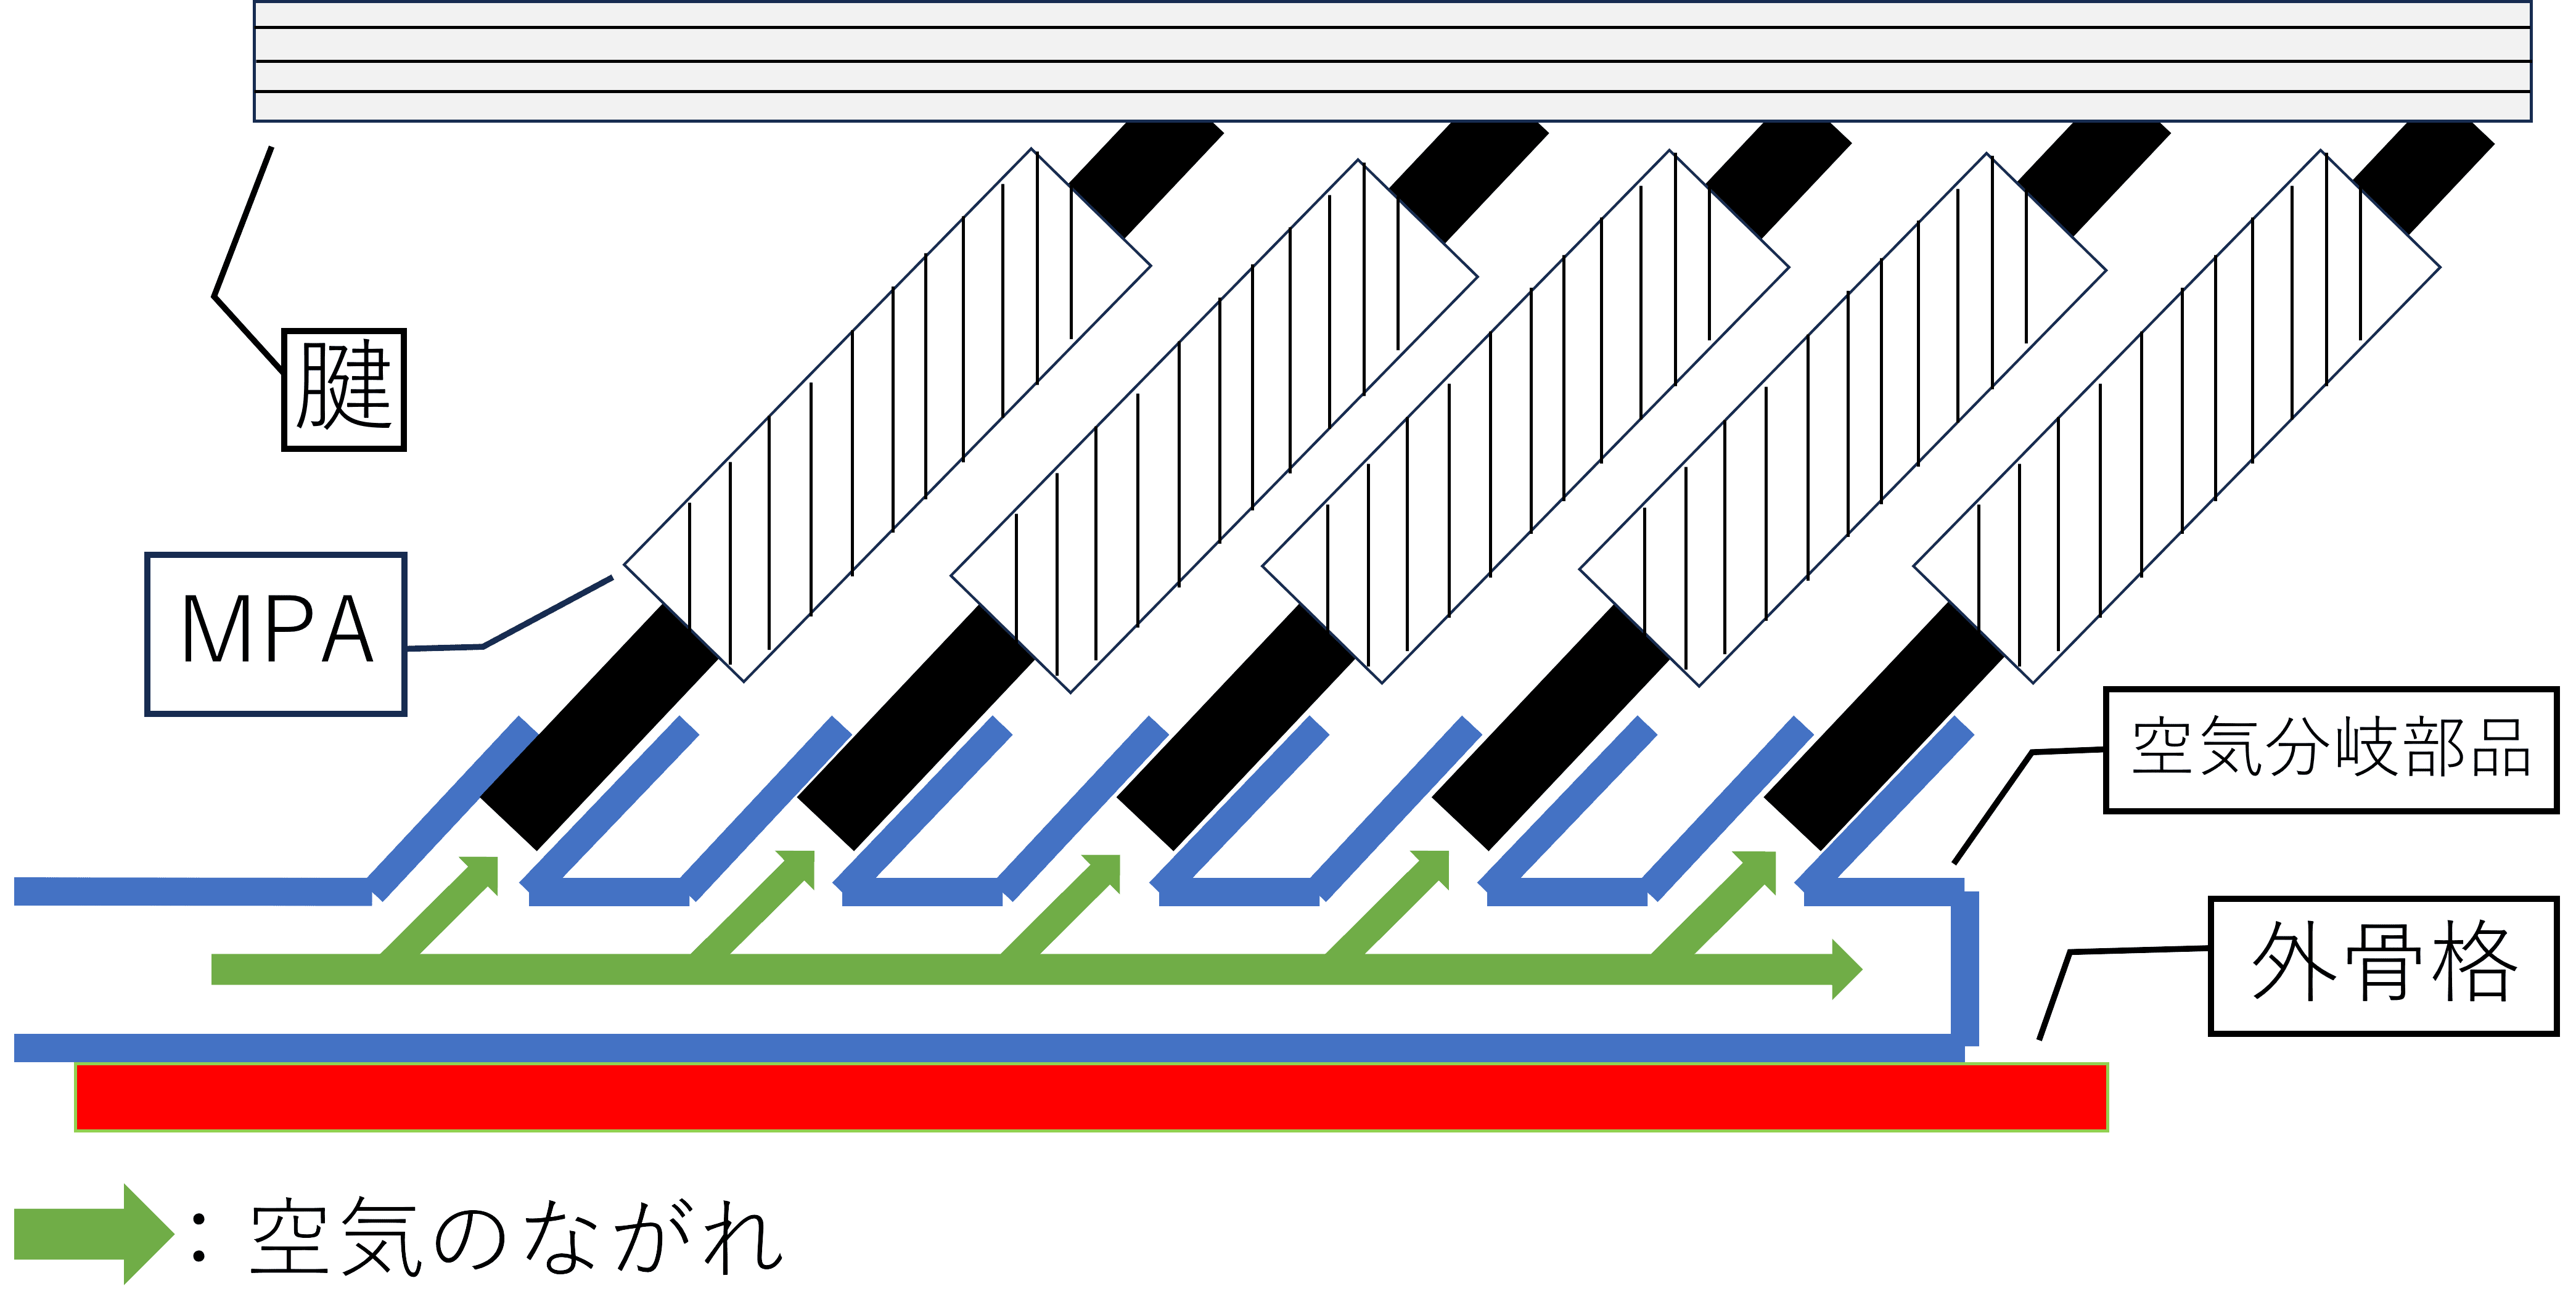
\includegraphics[scale=0.06]{image/air_moshiki.png}
    \subcaption{模式図}
    \label{fig:pmoshiki}
  \end{minipage}
  %
  \caption{予備実験に用いた集積部品}
  \label{fig:yobisyuseki}
\end{figure}
%
\begin{figure}[t]
  \begin{minipage}{1\hsize}
    \centering
    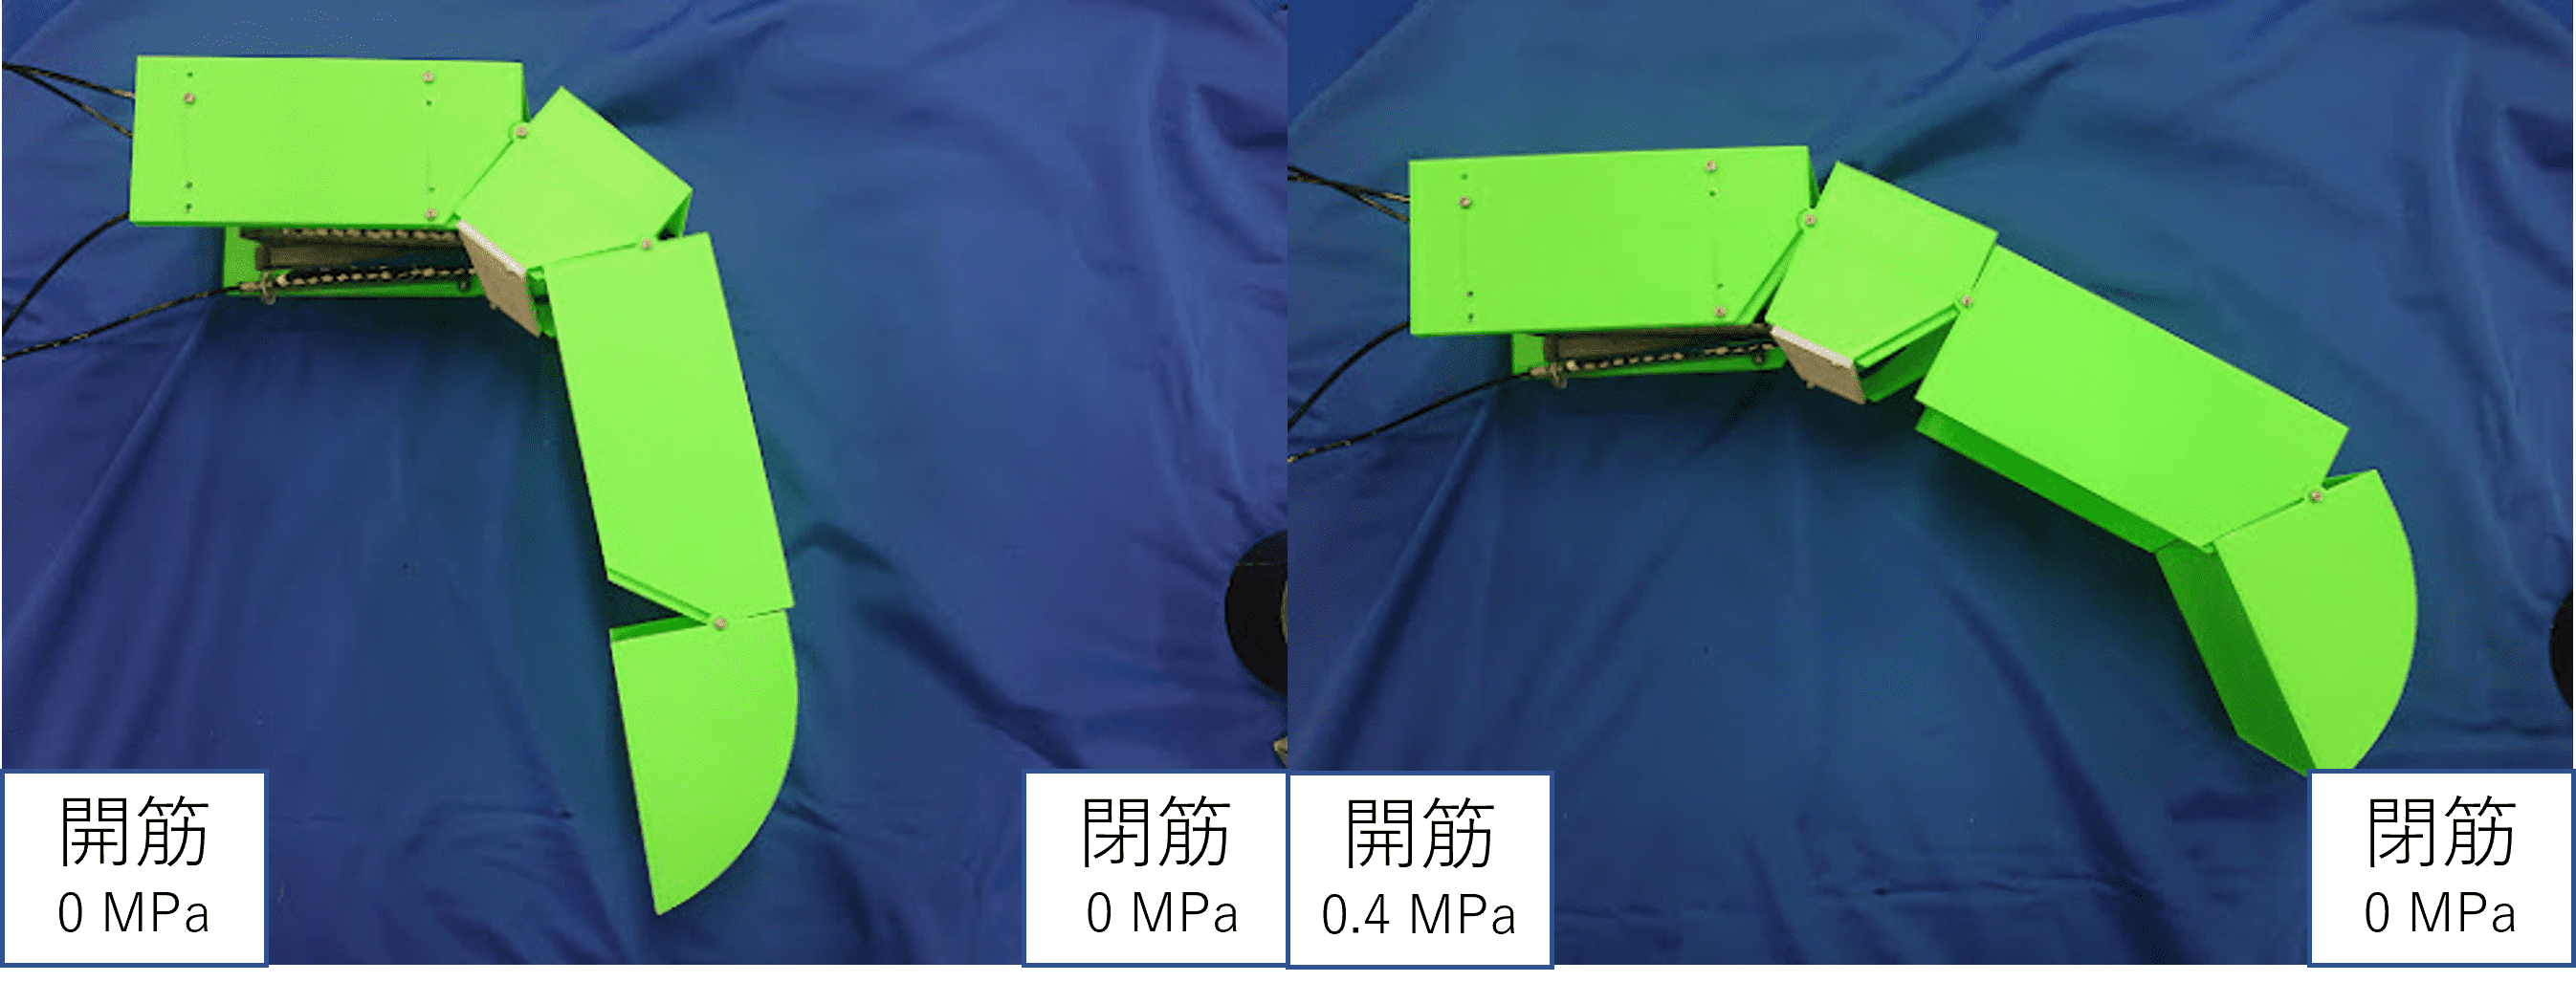
\includegraphics[scale=0.14]{image/yobi_open.png}
    \vspace{-1mm}
    \subcaption{開筋の動作}
    \label{fig:popen}
  \end{minipage}
  %
  \begin{minipage}{1\hsize}
    \centering
    \vspace{3mm}
    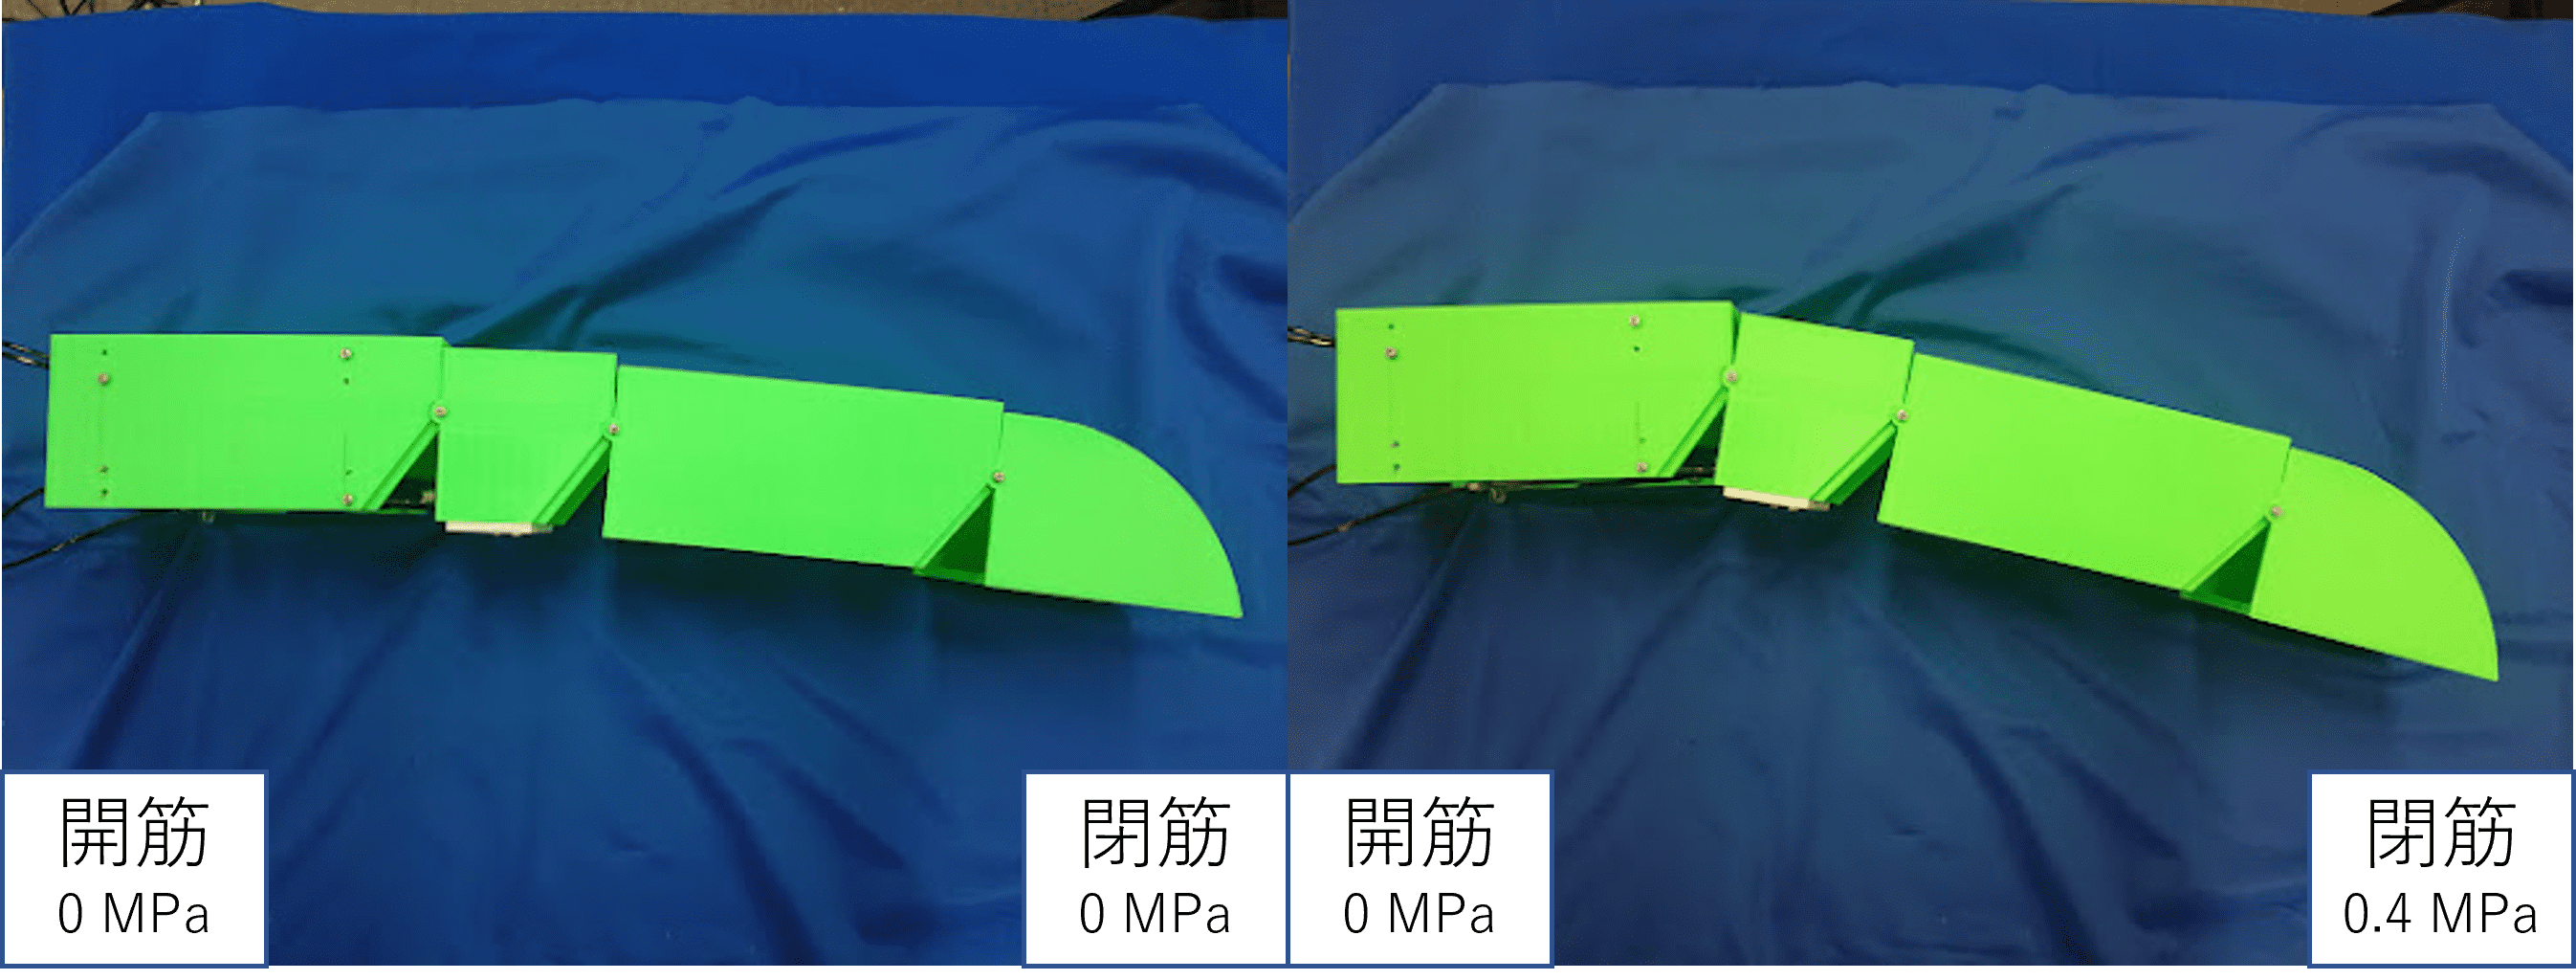
\includegraphics[scale=0.14]{image/yobi_close.png}
    \subcaption{閉筋の動作}
    \label{fig:pclose}
  \end{minipage}
  % \vspace{-5mm}
  \caption{予備実験}
  \label{fig:yobijikken}
\end{figure}
%%%%%%%%%%%%%%%%%%%%%%%%%%%%%%%%%%%%%%%%%%%%%%%%%%%%%%%%%
\subsection{予備実験}
\subsubsection{予備実験に用いた機体の構成}
MPAを羽状配置にした際の腱を引き込む動作を確認するために実験機を作製した.
実験機の外観を図\ref{fig:pkitai}に示す.
機体の大きさはMPAとその他部品が配置できる大きさとなっており,実際の蟹の比率とは異なる.
また,機体は4つの節に分かれているが腕節-前節間にあたる部分は実際の蟹の可動域とは異なるため,2次元3自由度の機体となっている.
各節は矩形状となっており,各節の連結にはネジを用いた.
腱の部分は硬さや柔軟性が類似しているプラスチック板を用いているがせん断に弱いためプラスチック板の周りはビニールテープによって補強をした.
%%%%%%%%%%%%%%%%%%%%%%%%%%%%%%%%%%%%%%%%%%%%%%%%%%%%%%%%%
%
%%%%%%%%%%%%%%%%%%%%%%%%%%%%%%%%%%%%%%%%%%%%%%%%%%%%%%%%%
\subsubsection{細径MPAの集積方法}
細径MPAの集積方法として,スライダレールの機構を参考にした集積方法を用いた.
図\ref{fig:yobisyuseki}\subref{fig:pken},\subref{fig:ptanbu},\subref{fig:pairtube}に作製した集積部品を示す.腱側の部品はアウターレールのようになっており,下部の隙間には腱となるプラスチック板を挿入できるようになっている(図\ref{fig:yobisyuseki}\subref{fig:pken}).
また,MPA端部はインナーレールのようになっている(図\ref{fig:yobisyuseki}\subref{fig:ptanbu}).
このように集積する際にMPAの本数が増えるため,一度にすべてのMPAに圧縮空気を印加することが可能な空気分岐部品(図\ref{fig:yobisyuseki}\subref{fig:pairtube})を作製した.
分岐部には角度がついており,この部品によって羽状筋の初期角度が決まる.
これらの集積部品を用いてMPAを集積した様子を図\ref{fig:yobisyuseki}\subref{fig:psyuseki}に示す.このように集積したMPAを反対側にもつけることで羽状筋を構成する.
空気分岐部品はネジ止めができるようになっており,外骨格とはネジ止めによって付着可能となっている.
集積したMPAの動作模式図を図\ref{fig:yobisyuseki}\subref{fig:pmoshiki}に示す.
%%%%%%%%%%%%%%%%%%%%%%%%%%%%%%%%%%%%%%%%%%%%%%%%%%%%%%%%%
\subsubsection{動作実験および結果}
羽状配置に集積したMPAを節を開く方向,閉じる方向へと配置し動作実験を行った.
実際の蟹の長節内部の羽状筋は回転軸に対して上下でなく左右に配置されているが,予備実験では上下の配置となっている.
予備実験ではMPAを羽状配置した際に動作することを確認することが目的なのでMPAは長節から腕節間にのみ配置した.
腱となるプラスチック板は腕節の端に張った状態となるようにビニールテープで固定し,初期位置は開筋,閉筋のどちらか一方の腱が張った状態としてから0.4 MPaを印可して動作実験を行った.

図\ref{fig:yobijikken}\subref{fig:popen},\subref{fig:pclose}に動作実験の結果を示す.
結果より,開筋に圧縮空気を印可した際は節の大きい動作が確認できたが,閉筋に印可した際には僅かな動作しか確認できなかった.
原因として羽状筋の角度が浅いことが挙げられる.
予備実験で用いた集積方法では一つ一つのMPAの長さが少しでも異なる場合,腱側の端部が干渉し,羽状筋の角度が浅くなっていた.
そのため腱を引き込む方向への力が小さくなり動作が小さくなったと考えられる.
また,予備実験の際に腱として用いていたプラスチック板は割れやすく,繰り返し荷重がかかると直ぐに破損してしまう問題点が確認された.
%%%%%%%%%%%%%%%%%%%%%%%%%%%%%%%%%%%%%%%%%%%%%%%%%%%%%%%%%
\subsection{3次元3自由度を有する歩脚ロボットの開発}
\subsubsection{機体の構成および寸法}
%%%%%%%%%%%%%%%%%%%%%%%%%%%%%%%%%%%%%%%%%%%%%%%%%%%%%%%%%
\begin{figure}[t]
  \begin{minipage}{1\hsize}
    \centering
    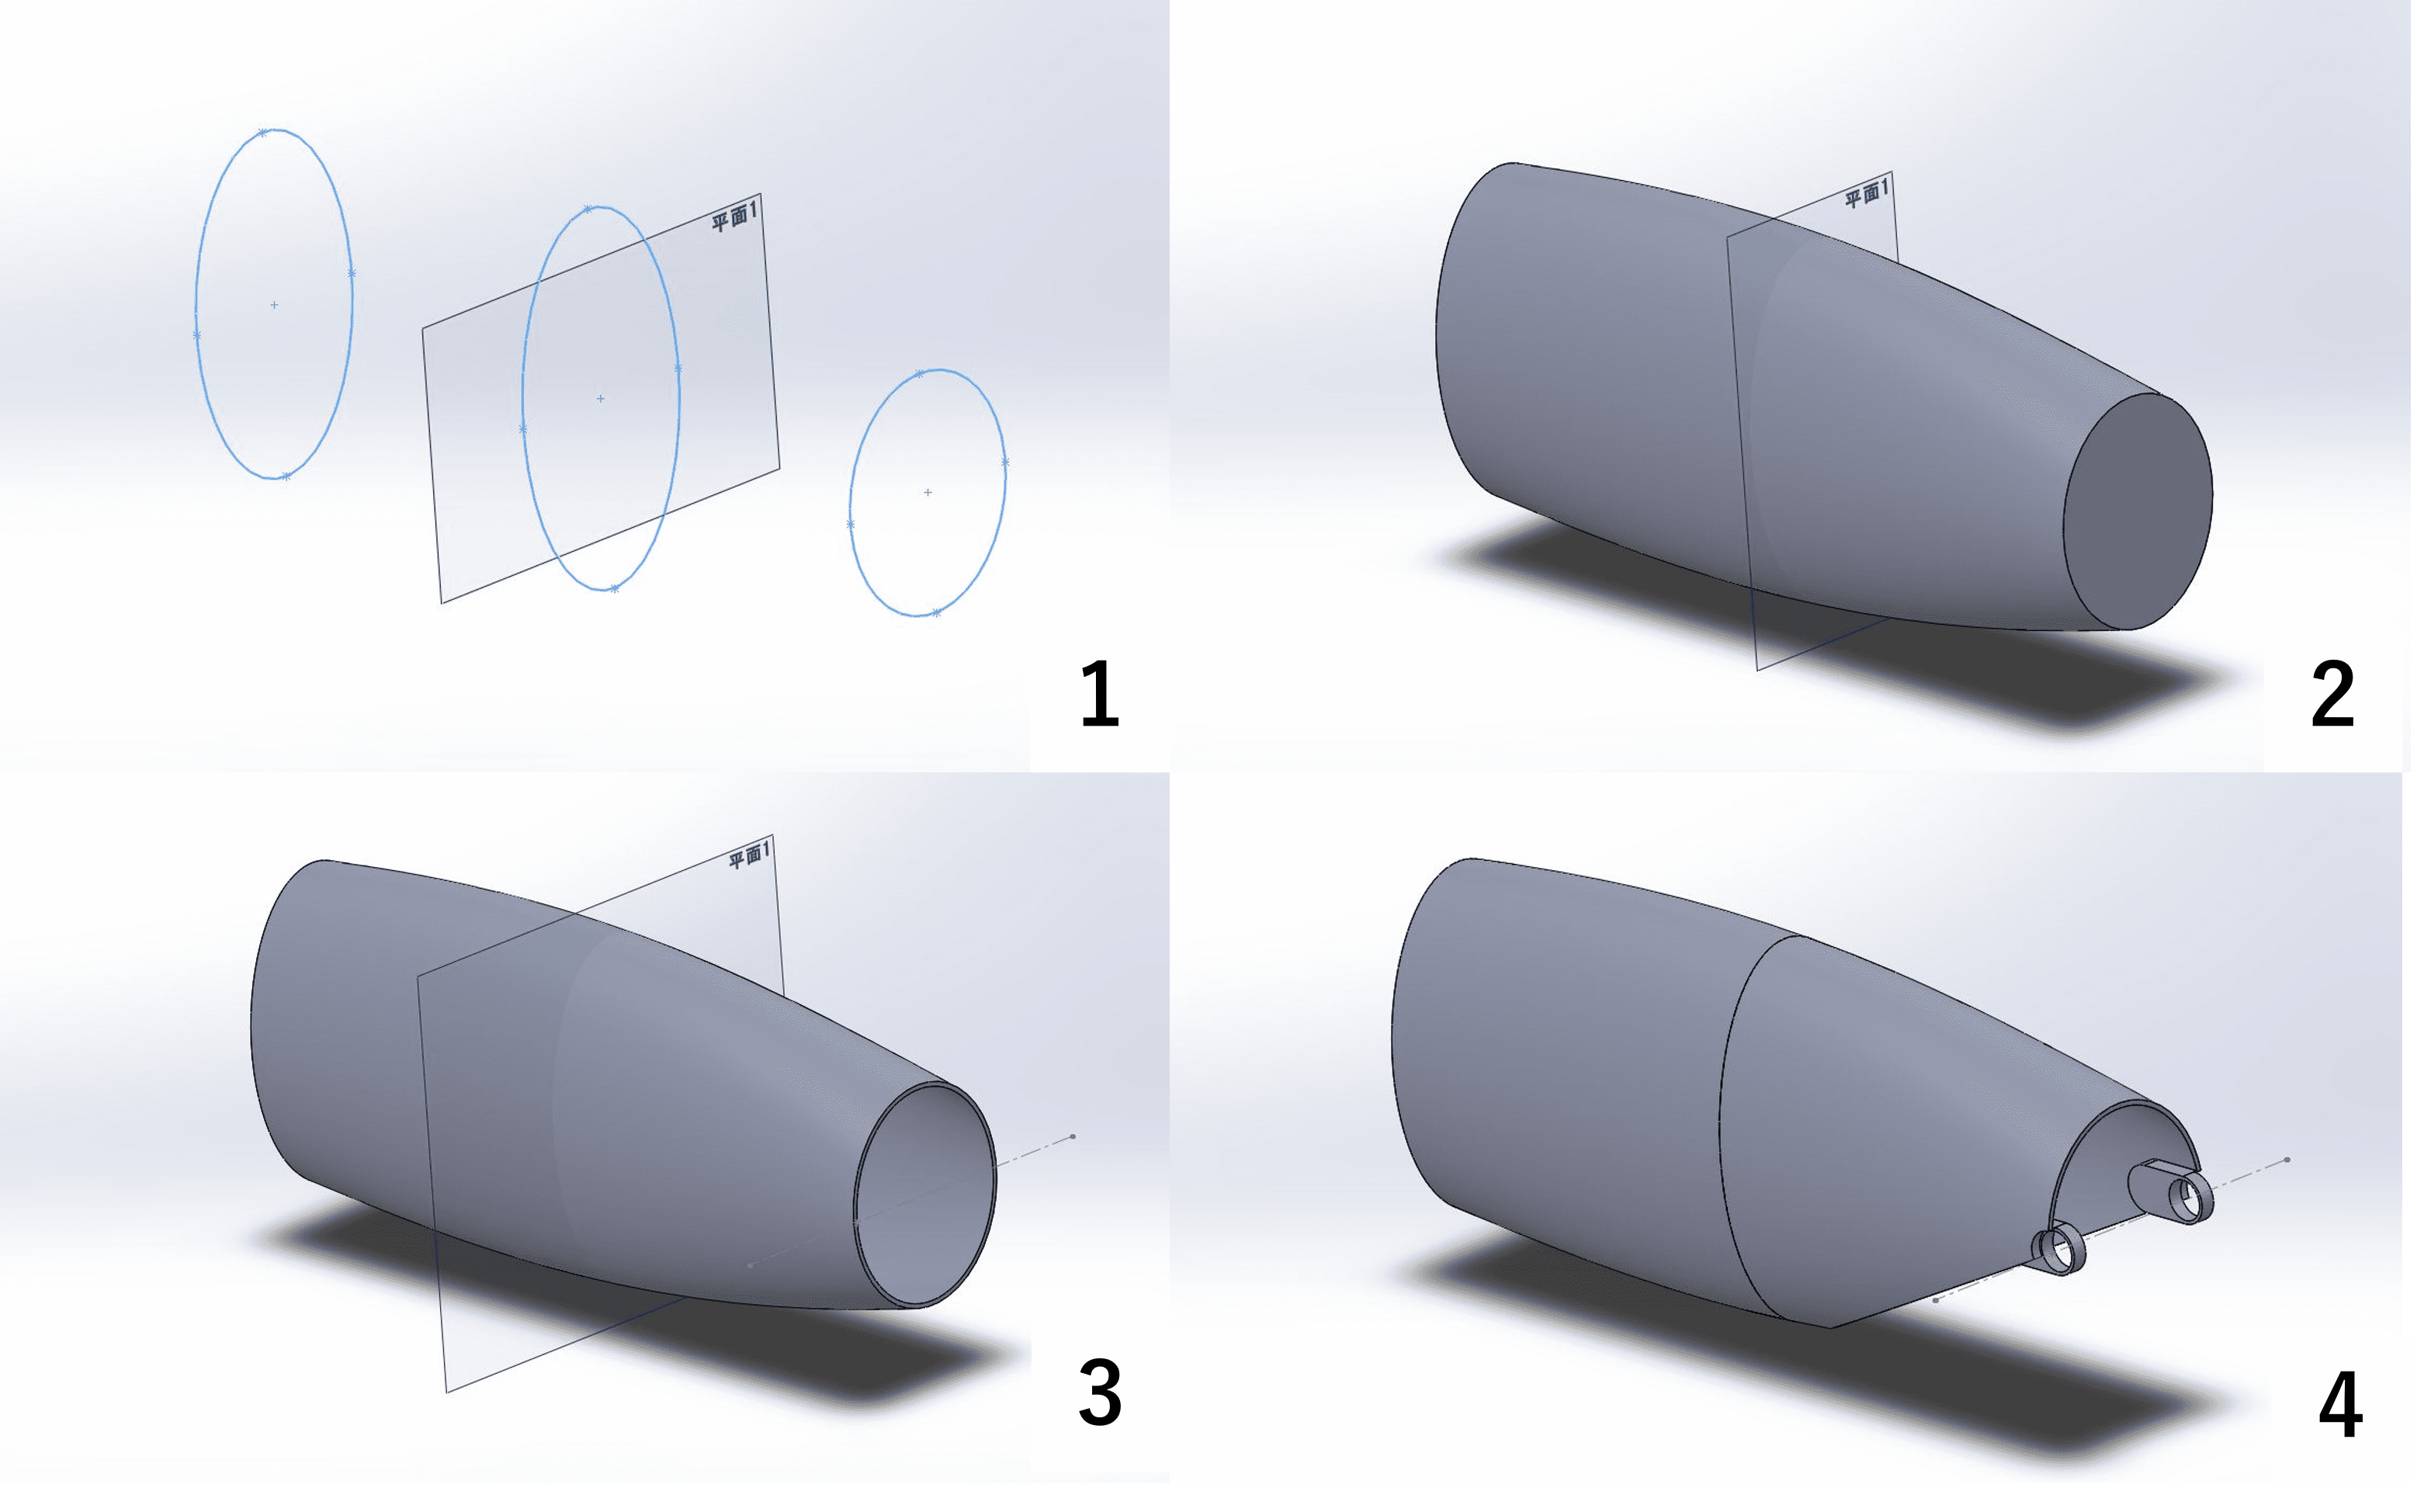
\includegraphics[scale=0.12]{image/kitaimethod.png}
    \caption{実機のSOLIDWORKS上での作製手順}
    \label{fig:solidw}
  \end{minipage}
\end{figure}
%
\begin{figure}[tbp]
  \centering
  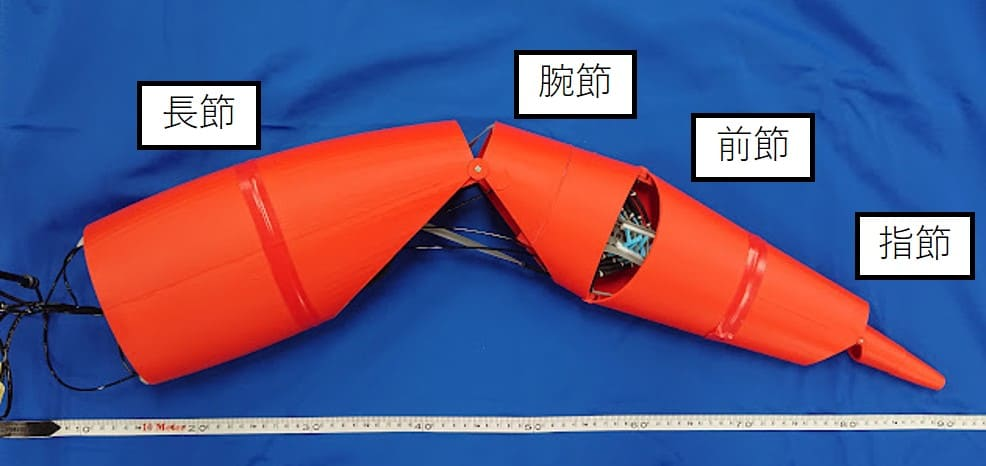
\includegraphics[scale=0.29]{image/robot_scale.JPG}
  \caption{ズワイガニの歩脚を模したロボット}
  \label{fig:jikki}
\end{figure}
%
\begin{figure}[t]
  \begin{minipage}{0.5\hsize}
    \centering
    \vspace{3mm}
    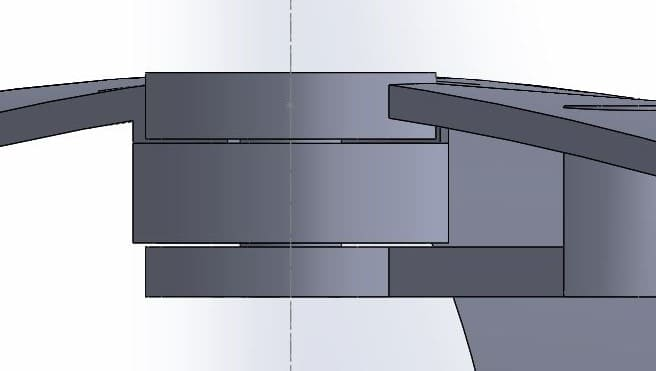
\includegraphics[scale=0.32]{image/bearingu.JPG}
    \subcaption{CAD図面(SOLIDWORKS)}
    \label{fig:bearingus}
  \end{minipage}
  %
  \begin{minipage}{0.5\hsize}
    \centering
    \vspace{7mm}
    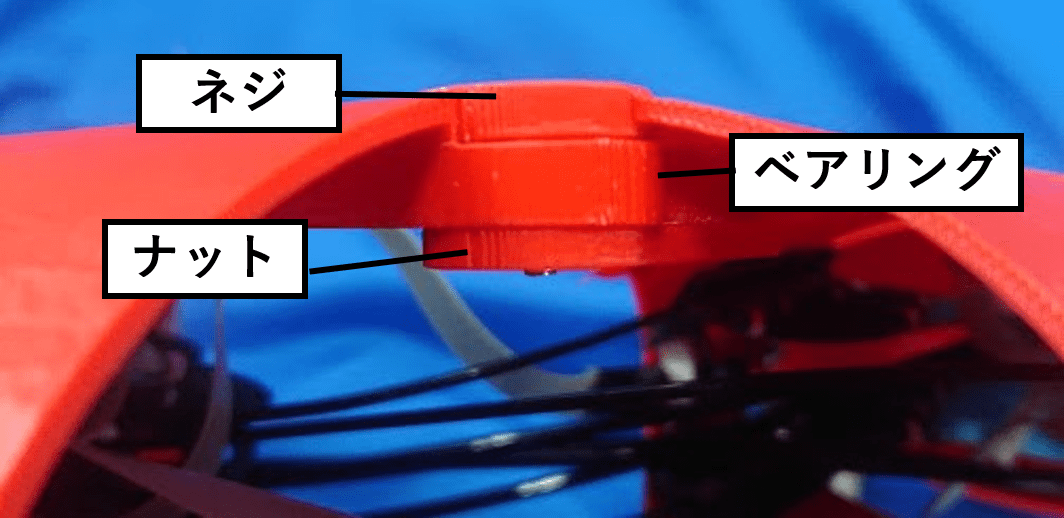
\includegraphics[scale=0.2]{image/bearinguj.png}
    \subcaption{実物}
    \label{fig:bearinguj}
  \end{minipage}
  \caption{関節構造}
  \label{fig:bearingu}
\end{figure}
%%%%%%%%%%%%%%%%%%%%%%%%%%%%%%%%%%%%%%%%%%%%%%%%%%%%%%%%%
実際の蟹の寸法や可動域などをもとにした3次元3自由度を有する歩脚ロボットの機体について述べる.
本研究では解剖時に測定したズワイガニの最も大きい歩脚(第4肢)について表\ref{tab:4setu},表\ref{tab:4setukadou}に示した寸法および可動域を基に機体を作製した.
図\ref{fig:solidw}に3DCADソフトのSOLIDWORKSを用いた機体の設計方法を示す.
以下,設計手順である.
%%%%%%%%%%%%%%%%%%%%%%%%%%%%%%%%%%%%%%%%%%%%%%%%%%%%%%%%%
\vspace{3mm}
\begin{enumerate}
  \item 測定した寸法を基に2~3個の楕円輪郭を描く
  \item 描いた楕円輪郭をロフトで繋ぎ,立体にする(ロフト:2つ以上の輪郭を繋ぎ立体的な形状を作る機能)
  \item シェルを用いて立体を厚み2 mmでくり抜く(シェル:指定した面を開けて均一な厚みにくり抜く機能)
  \item 測定した可動域を実現できるよう端面をカットし,端部にベアリングを挿入できるように加工
\end{enumerate}
%%%%%%%%%%%%%%%%%%%%%%%%%%%%%%%%%%%%%%%%%%%%%%%%%%%%%%%%%
以上の手順で作製した機体を図\ref{fig:jikki}に示す.
寸法については表\ref{tab:4setu}に示した実測値を小数点以下で切り捨て,直径方向へ7倍,長手方向へ3.5倍のサイズとした.
ただし,直径方向へは集積部品の厚みも考慮して5 mm加えた.
外殻の厚みは一律で2 mmとなっている.
また,手順にもあるように関節部にはベアリングを使用した(図\ref{fig:bearingu}\subref{fig:bearingus},\subref{fig:bearinguj}).
具体的な機体の寸法を表\ref{tab:scalej}に,使用したベアリングの寸法を表\ref{tab:bearingu}に示す.
機体の作製にはFDM方式の3Dプリンタを使用し,印刷の際は各節を半分にしてからそれぞれ出力した.
%%%%%%%%%%%%%%%%%%%%%%%%%%%%%%%%%%%%%%%%%%%%%%%%%%%%%%%%%
\begin{table}[t]
  \begin{minipage}{1\hsize}
    \centering
    \caption{実機寸法}
    \label{tab:scalej}
    \vspace{-3mm}
    \begin{tabular}{|c|c|c|c|c|}
    \hline
      & 左 [mm]         & 中 [mm]         & 右 [mm]         & 長手方向 [mm] \\ \hline
    長節 & 137.5-81.5 & 151.5-81.5 & 95.5-81.5  & 350  \\ \hline
    腕節 & 95.5-81.5  & -          & 130.5-60.5 & 140  \\ \hline
    前節 & 130.5-60.5 & -          & 74.5-32.5  & 245  \\ \hline
    指節 & 35.5-32.5  & -          & -          & 100  \\ \hline
    \end{tabular}
  \end{minipage}
  %
  \begin{minipage}{1\hsize}
    \centering
    \vspace{3mm}
    \caption{ベアリングの各寸法}
    \vspace{-3mm}
    \label{tab:bearingu}
    \begin{tabular}{|c|c|c|c|c|}
    \hline
          & 外径 [mm] & 内径 [mm]  & 厚み [mm]  & ネジ,ナット \\ \hline
    長節-腕節間 & 16 & 4   & 6   & M3      \\ \hline
    腕節-前節間 & 8  & 3   & 4   & M3      \\ \hline
    前節-指節間 & 6  & 2.5 & 2.6 & M2      \\ \hline
    \end{tabular}
  \end{minipage}
\end{table}
%%%%%%%%%%%%%%%%%%%%%%%%%%%%%%%%%%%%%%%%%%%%%%%%%%%%%%%%%
\begin{figure}[t]
  \begin{minipage}{0.5\hsize}
    \centering
    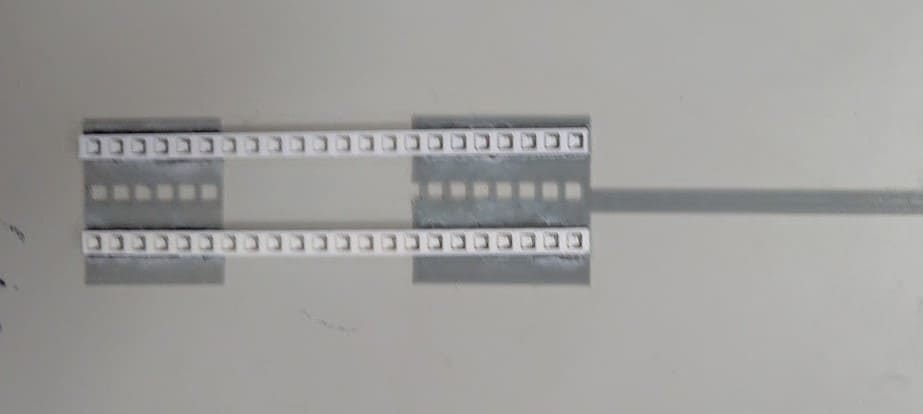
\includegraphics[scale=0.2]{image/ken.JPG}
    \subcaption{腱部品}
    \label{fig:jken}
  \end{minipage}
    %
  \begin{minipage}{0.5\hsize}
    \centering
    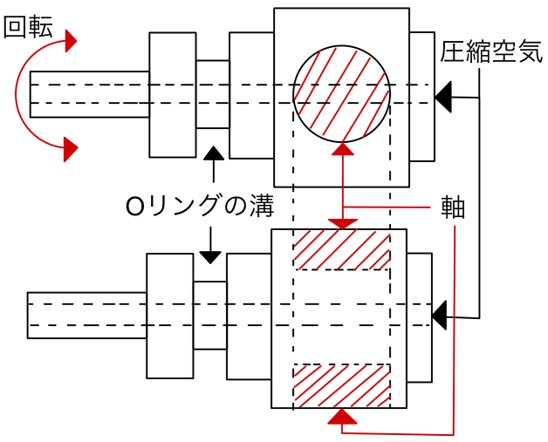
\includegraphics[scale=0.3]{image/MPA_tanbu.JPG}
    \subcaption{MPA端部}
    \label{fig:jtanbu}
  \end{minipage}
    %
  \begin{minipage}{0.5\hsize}
    \vspace{3mm}
    \centering
    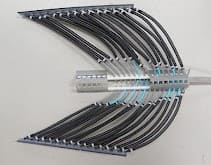
\includegraphics[scale=0.6]{image/syuseki.JPG}
    \subcaption{羽状筋状に集積した様子}
    \label{fig:jsyuseki}
  \end{minipage}
    %
    \hspace{-5mm}
  \begin{minipage}{0.5\hsize}
    \centering
    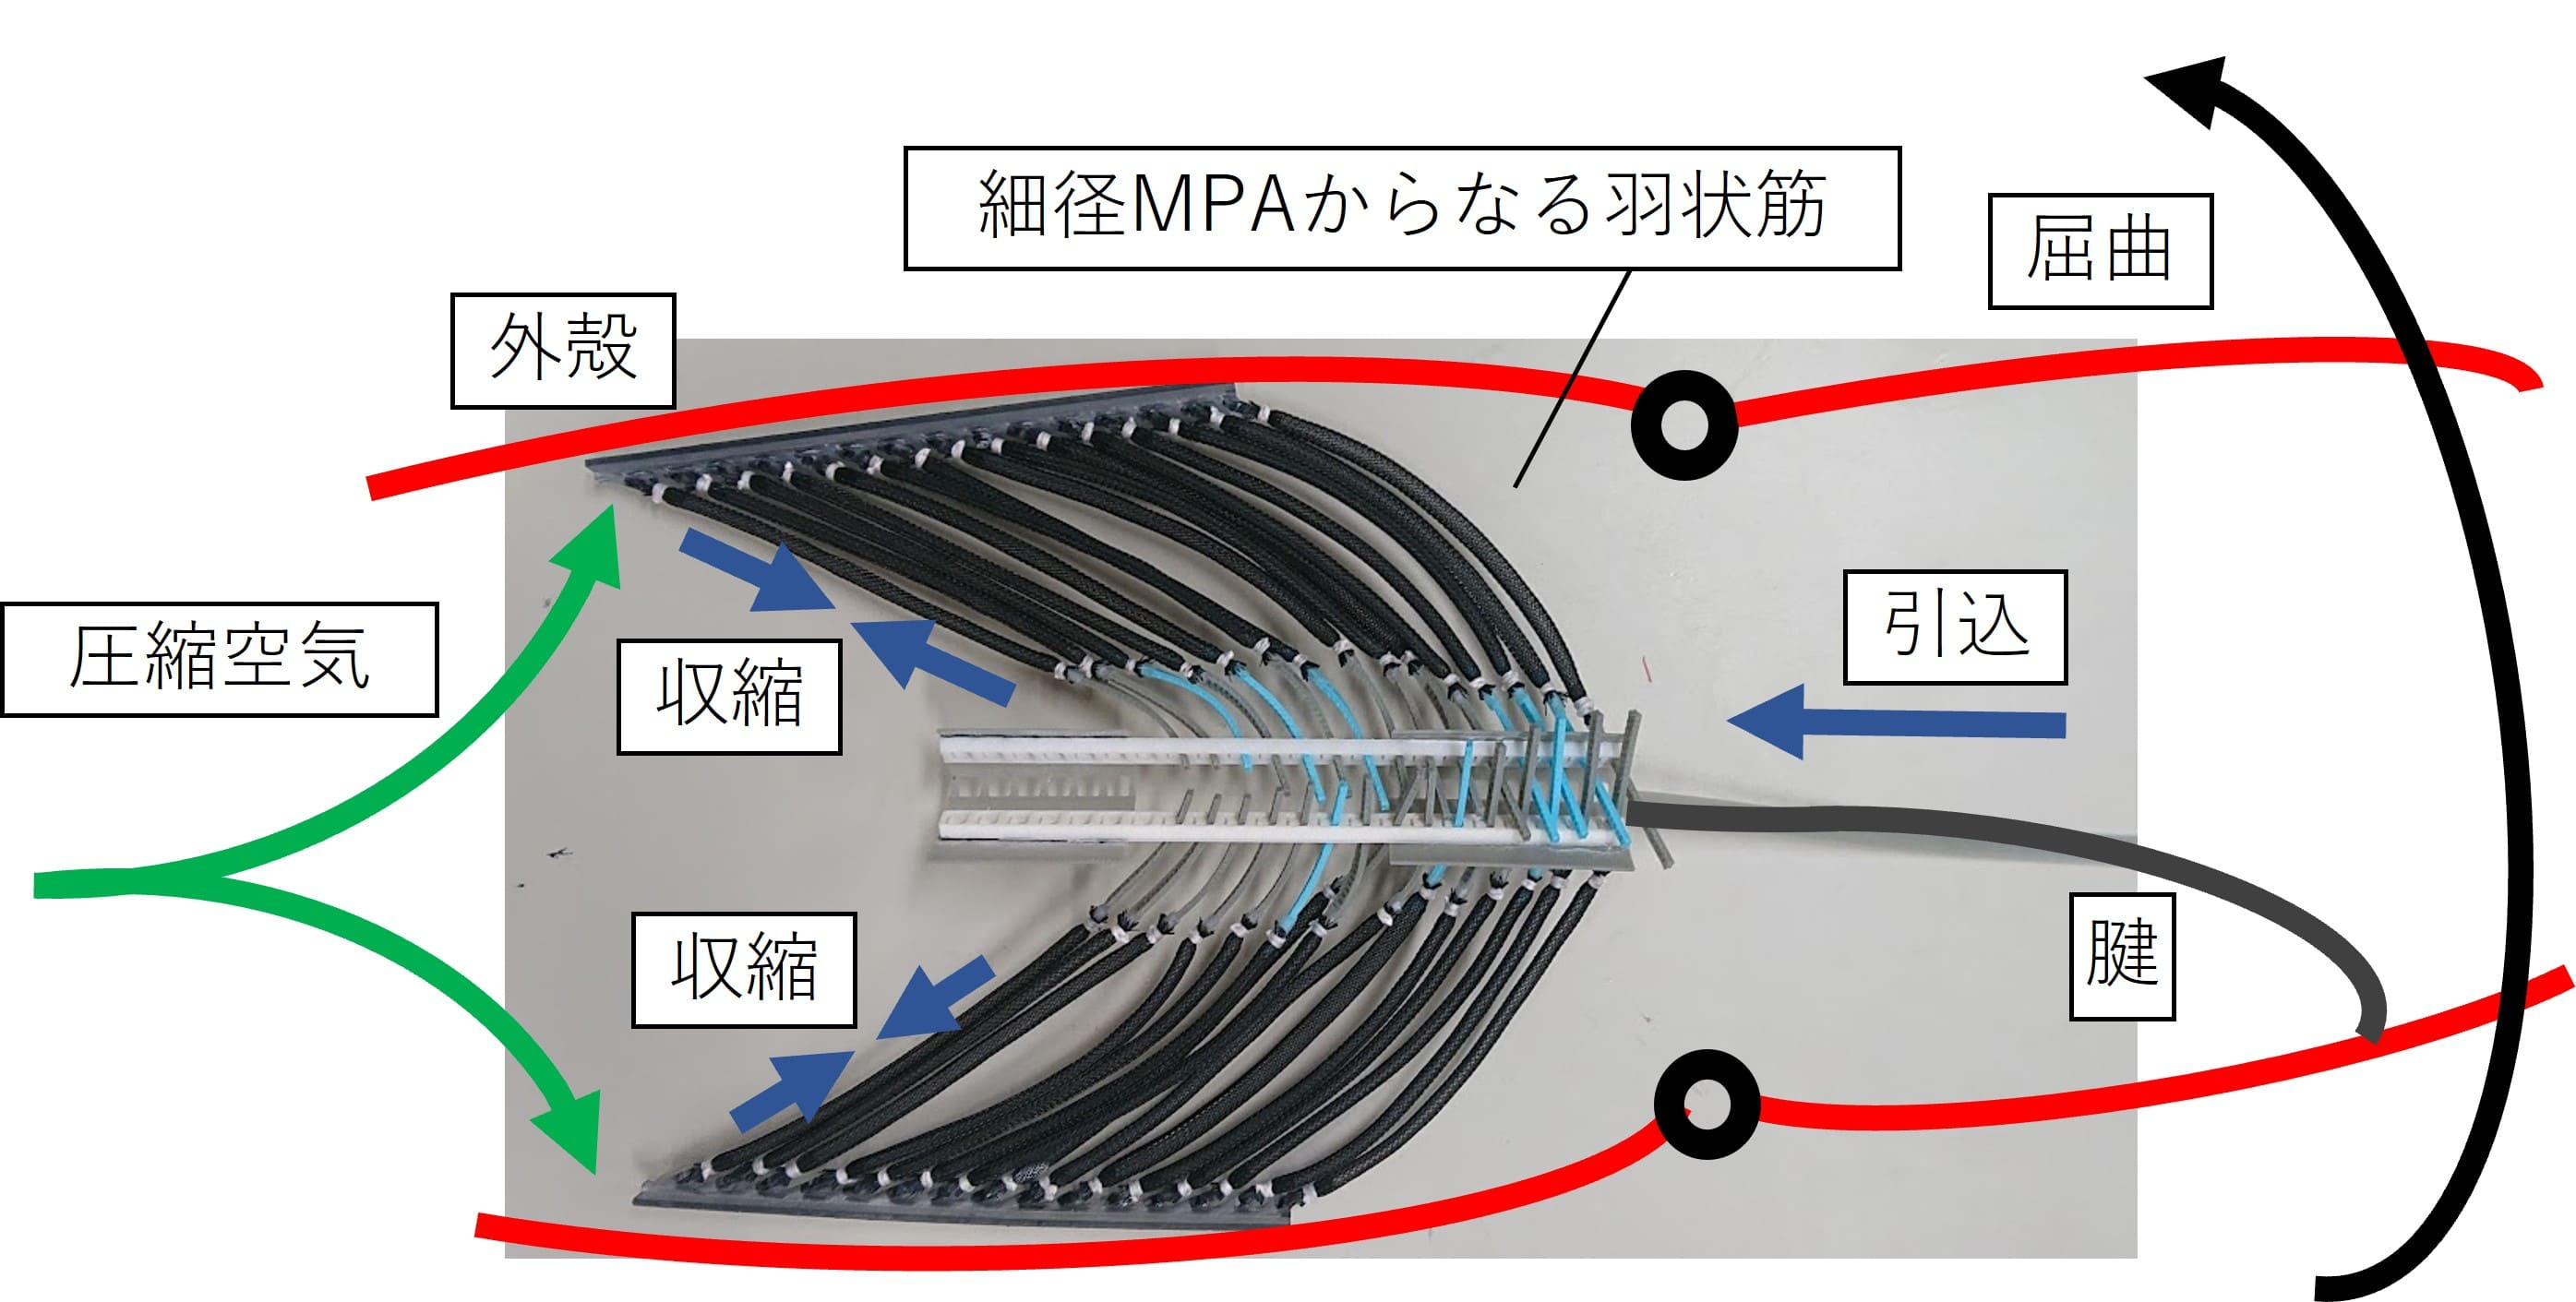
\includegraphics[scale=0.07]{image/mosiki.JPG}
    \subcaption{模式図}
    \label{fig:jmosiki}
  \end{minipage}
    %
  \caption{改良した集積方法}
  \label{fig:syusekijikki}
\end{figure}
    %
\begin{figure}[t]
  \begin{minipage}{0.5\hsize}
    \centering
    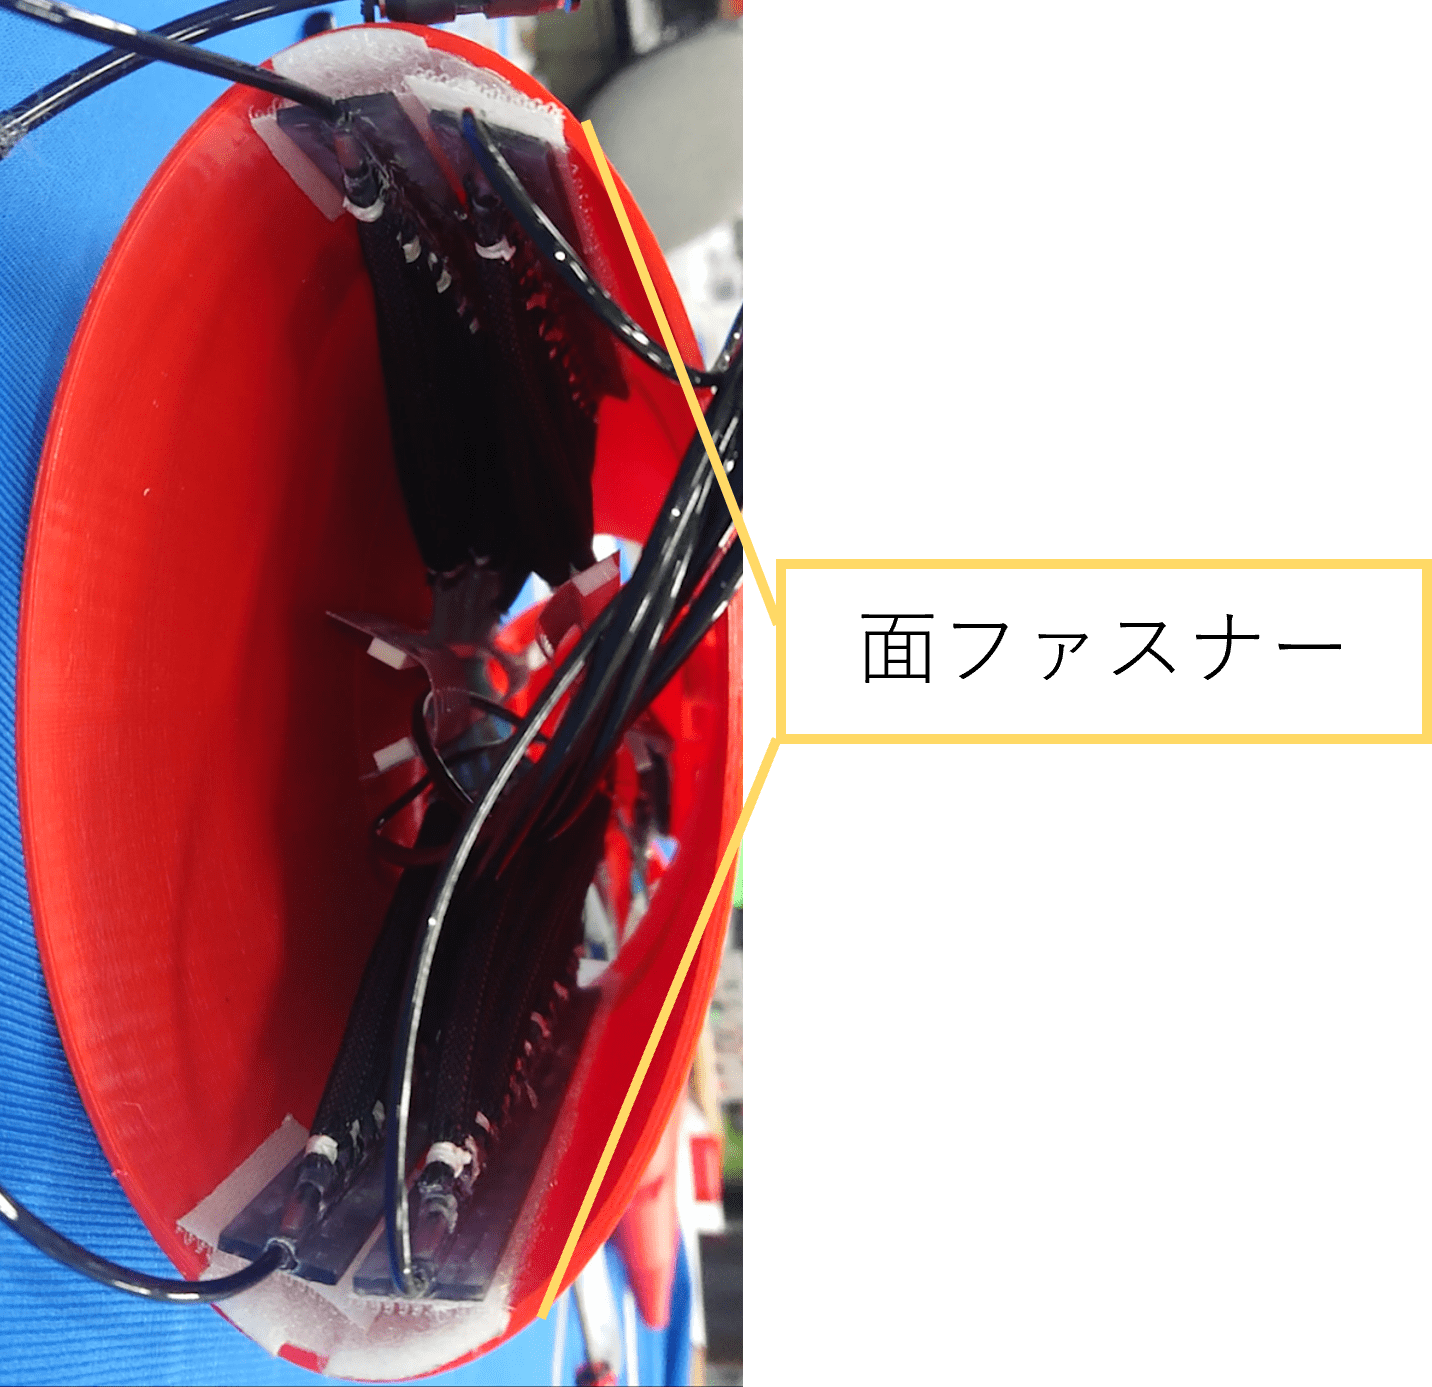
\includegraphics[scale=0.09]{image/syusekikotei.png}
    \caption{外殻との付着方法}
    \label{fig:syusekikotei}
  \end{minipage}
    %
  \begin{minipage}{0.5\hsize}
    \centering
    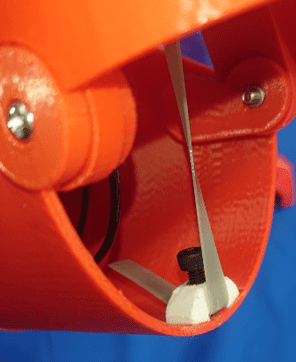
\includegraphics[scale=0.35]{image/kenkotei.png}
    \caption{腱の外殻への固定方法}
    \label{fig:kenkotei}
  \end{minipage}
\end{figure}
%%%%%%%%%%%%%%%%%%%%%%%%%%%%%%%%%%%%%%%%%%%%%%%%%%%%%%%%%
\subsubsection{改良したMPAの集積方法}
ズワイガニを模した機体では予備実験に用いた機体よりも内部のスペースが限られたため,よりコンパクトに羽状配置を構成できるような集積方法を用いる必要があった.
また,予備実験に用いた集積方法ではMPA一つ一つの長さが異なると羽状配置が崩れるため,本研究で用いる手作業で作製するMPAには不向きな集積方法であった.
これらの問題を解決するために取り付けと長さの調節が容易な結束バンドの機構に注目し集積部品を作製した.
図\ref{fig:syusekijikki}\subref{fig:jken},\subref{fig:jtanbu}のようにMPA端部はTPU素材で結束バンドのシート部にし,腱部分はPLA素材で結束バンドのヘッド部を連結させたような形状にすることで長さの調節が可能かつ強固に固定できる集積方法となっている.
腱部分のPLA部品の連結には予備実験に用いたプラスチック板よりも剛性に優れている穴の開いたTPU素材のシートを用いることで立体的に集積できるようになっており,シートの端部を細長く伸ばすことで隣の節まで繋げられるようになっている.

図\ref{fig:syusekijikki}\subref{fig:jsyuseki}に実際に集積したMPAを示す.
また,図\ref{fig:syusekijikki}\subref{fig:jmosiki}に機体に配置した際の動作の模式図を示す.
本来,羽状筋は立体的に配置されているが機体内部のスペースに限りがあるため上下の2方向から羽状筋を構成した.
集積したMPAと外殻の付着には容易に着脱可能かつ強固に固定可能な面ファスナーを用いた(図\ref{fig:syusekikotei}).本研究では空気分岐部品の裏面に面ファスナーのフック側,外殻にループ側を取り付けることで着脱できるようになっている.
腱と外殻の付着にはインサートナットを使用している.
外殻とは別でインサートナット挿入部品をFDM方式方式の3Dプリンタで作製し,インサートナット挿入後,外殻へ瞬間接着剤(PPX メーカー:セメダイン 品番:CA-522)を用いて固定した.
その後,インサートナットと外殻の隙間にTPUシートを挿入し,ネジ止めすることで固定可能となっている.
%%%%%%%%%%%%%%%%%%%%%%%%%%%%%%%%%%%%%%%%%%%%%%%%%%%%%%%%%
\begin{figure}[tbp]
  \begin{minipage}{1\hsize}
    \centering
    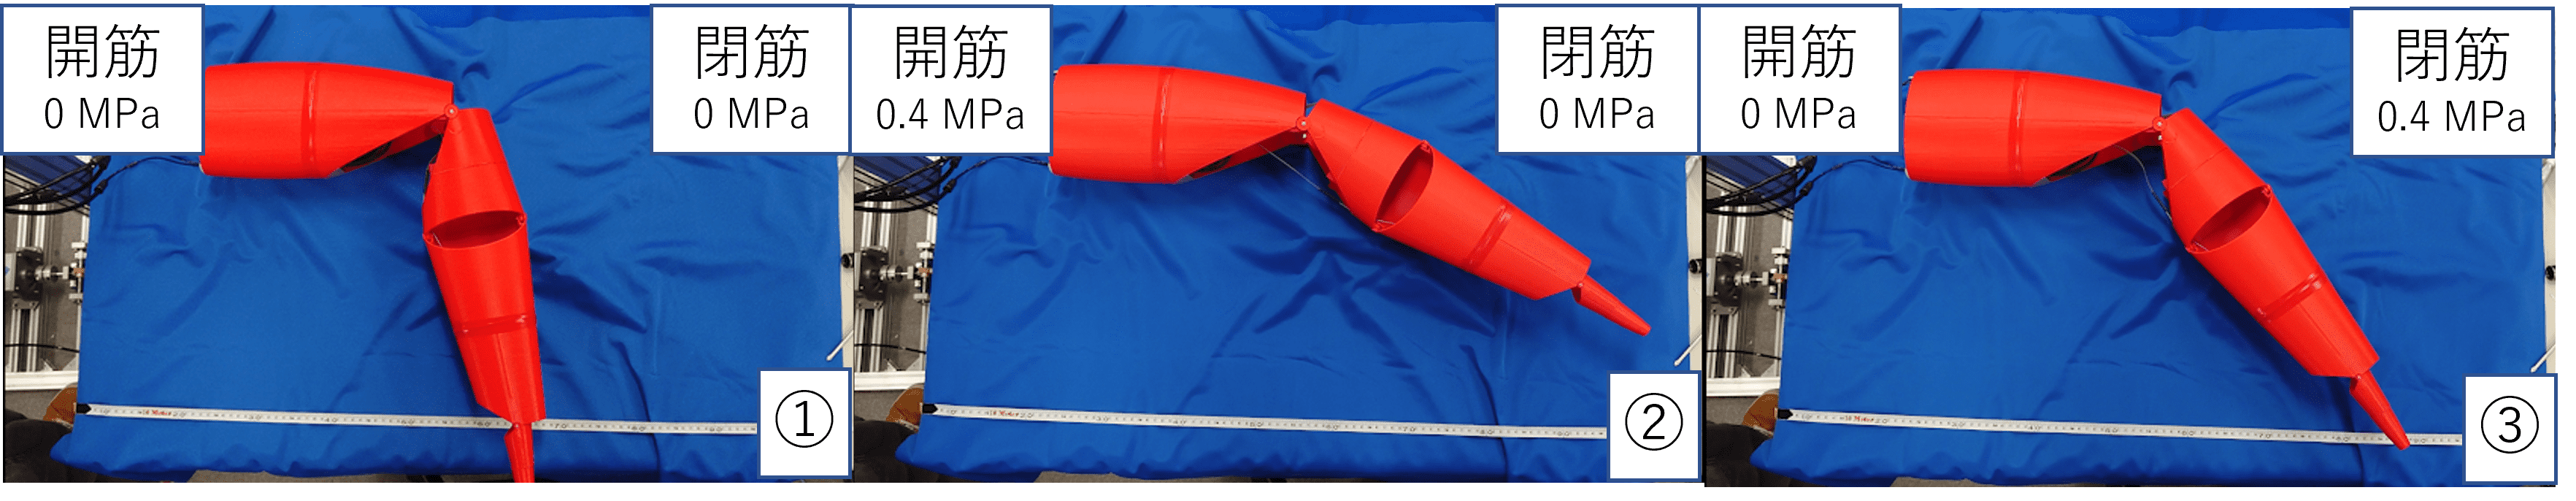
\includegraphics[scale=0.12]{image/move1all.png}
    \subcaption{長節-腕節間の動作}
    \label{fig:move1all}
  \end{minipage}
  %
  \begin{minipage}{1\hsize}
    \centering
    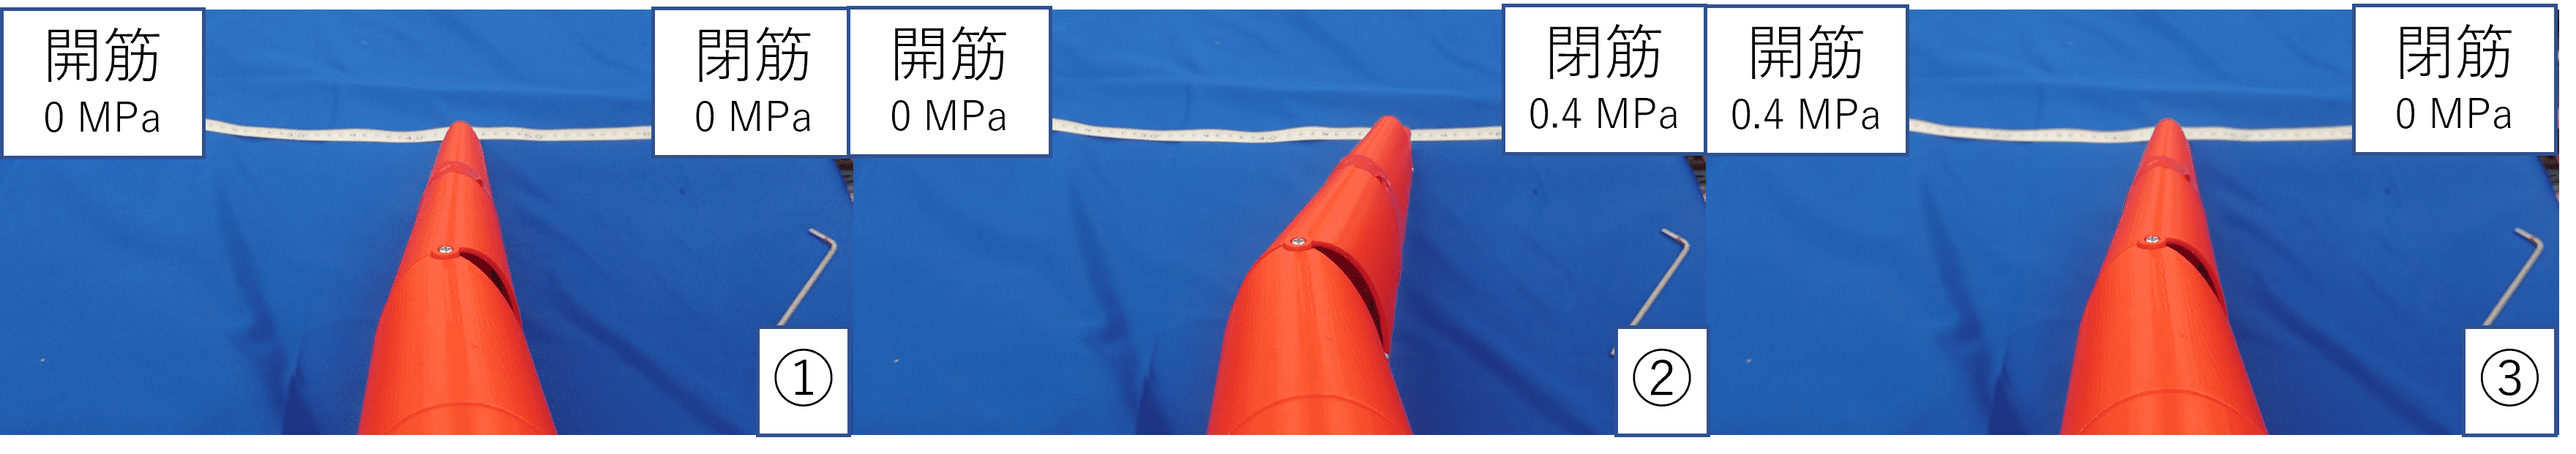
\includegraphics[scale=0.12]{image/move2all.png}
    \subcaption{腕節-前節間の動作}
    \label{fig:move2all}
  \end{minipage}
%
  \caption{動作実験}
  \label{fig:moveall}
\end{figure}
%%%%%%%%%%%%%%%%%%%%%%%%%%%%%%%%%%%%%%%%%%%%%%%%%%%%%%%%%
\begin{figure}[t]
    \centering
    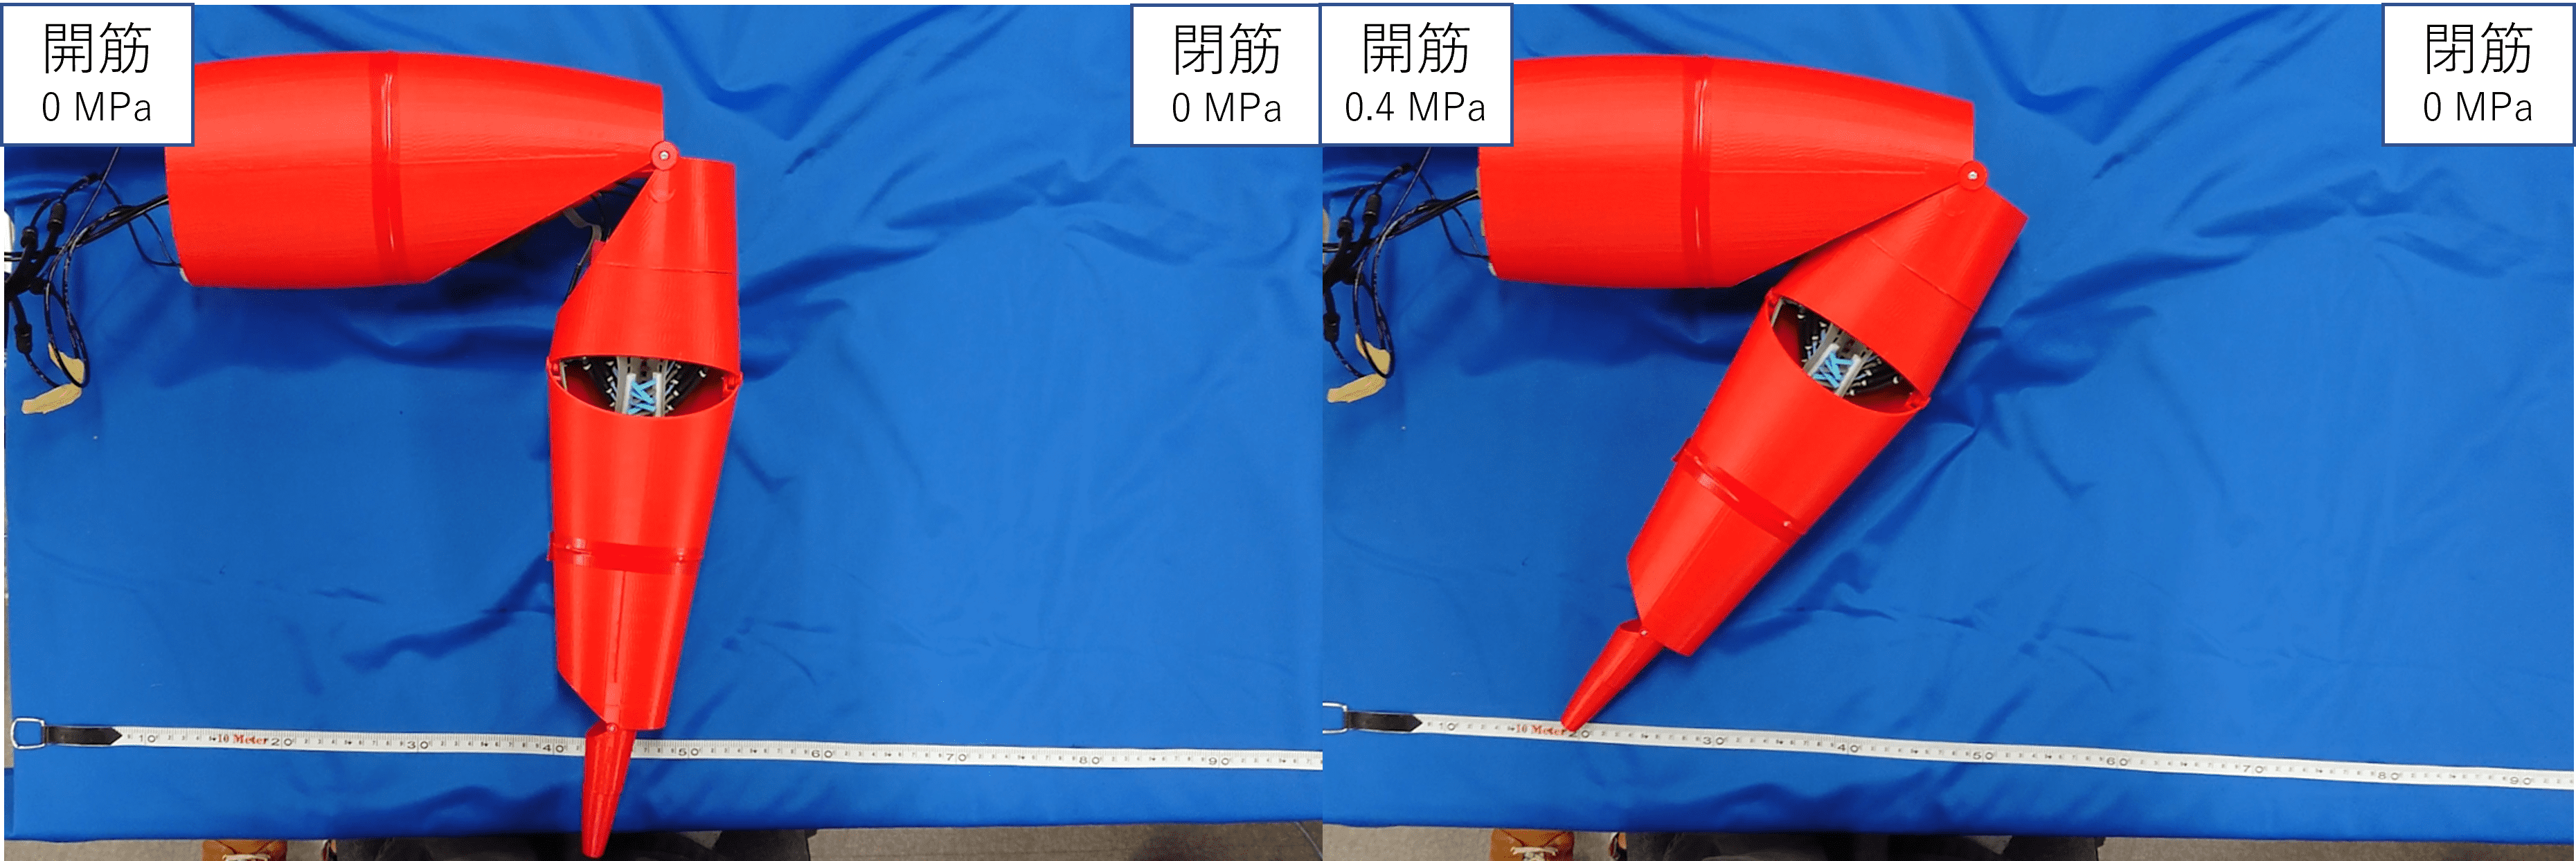
\includegraphics[scale=0.12]{image/kousatu1.png}
    \caption{角度による動作の変化}
    \label{fig:kousatu1}
\end{figure}
%
\begin{figure}[t]
  \begin{minipage}{0.5\hsize}
    \centering
    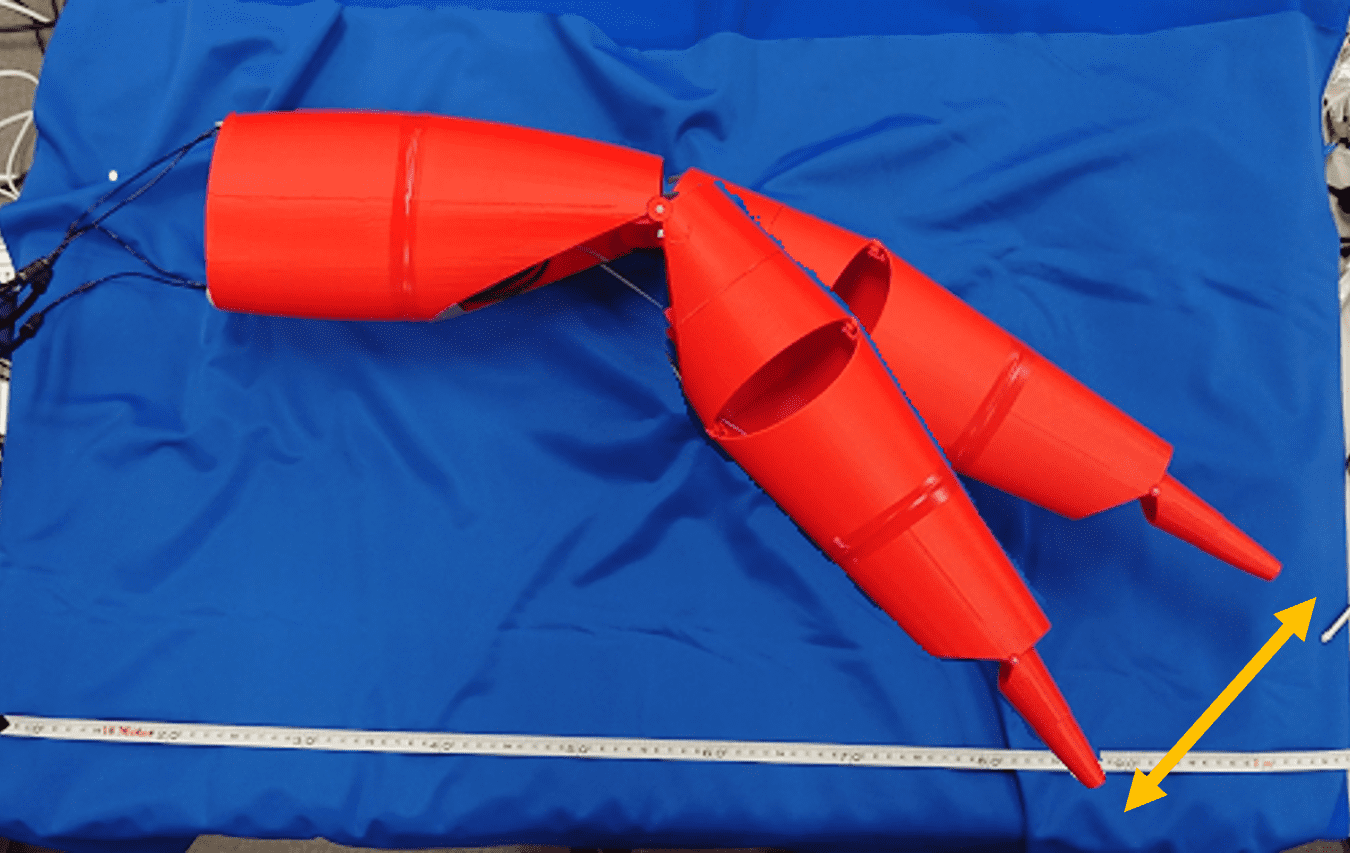
\includegraphics[scale=0.15]{image/kousatu2_1.png}
    \subcaption{長節-腕節間の駆動範囲}
    \label{fig:kousatu2_1}
  \end{minipage}
  %
  \begin{minipage}{0.5\hsize}
    \centering
    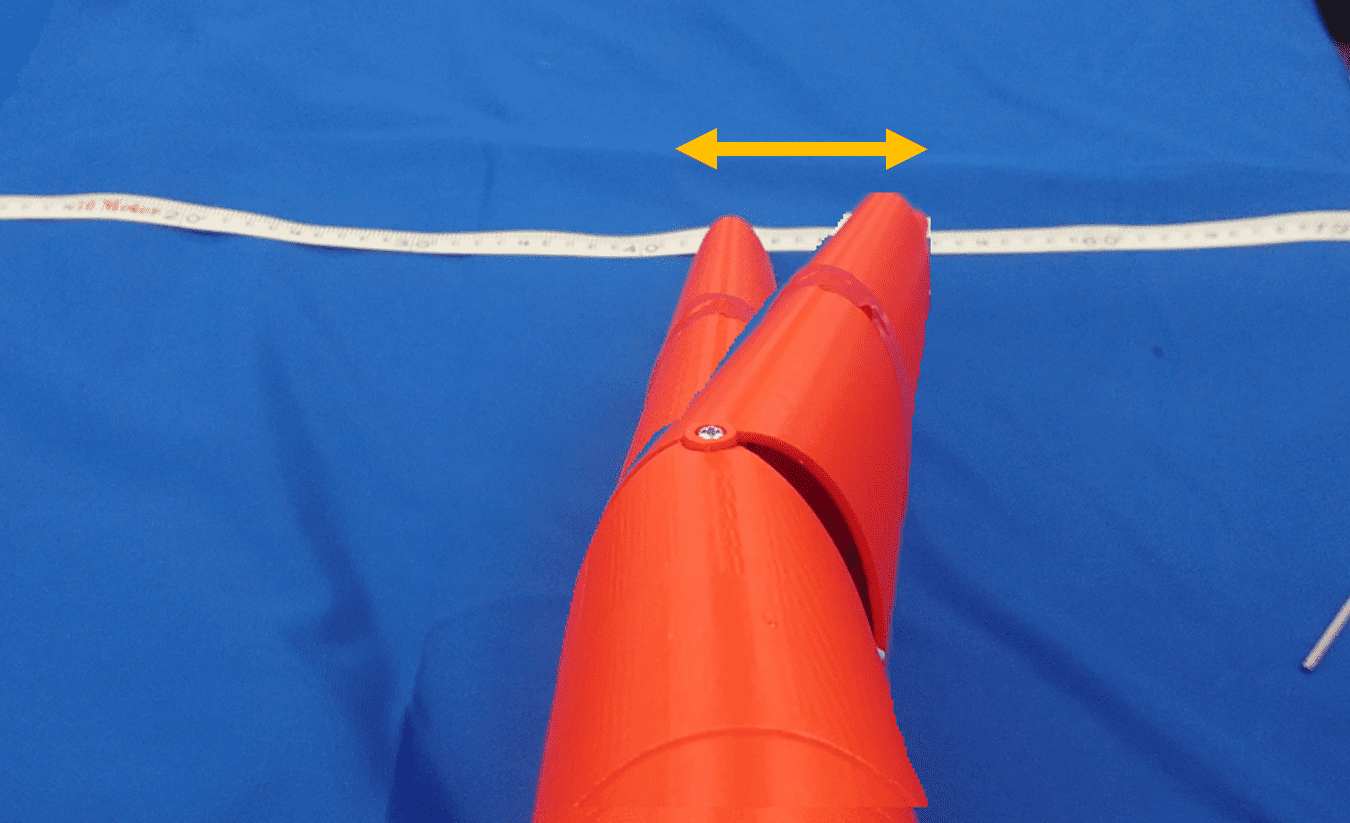
\includegraphics[scale=0.15]{image/kousatu2_2.png}
    \subcaption{腕節-前節間の駆動範囲}
    \label{fig:kousatu2_2}
  \end{minipage}
  %
  \caption{駆動範囲}
  \label{fig:kousatu2}
\end{figure}
%%%%%%%%%%%%%%%%%%%%%%%%%%%%%%%%%%%%%%%%%%%%%%%%%%%%%%%%%
\subsubsection{動作実験および結果}
羽状配置に集積したMPAを長節から腕節,腕節から前節間の開筋,閉筋に配置し動作実験を行った.
関節の動きを確認しやすくするために長節-腕節間は機体を寝かせた状態,腕節-前節間は機体を立てた状態で動作実験を行った.
また,初期位置は開筋か閉筋のどちらか一方の腱が張った状態の位置とし,空気の印加は手動で行い印加圧力は0.4 MPa,開筋と閉筋の手動弁を交互に開閉させることで動作させた.

長節-腕節間の動作結果を図\ref{fig:moveall}\subref{fig:move1all},腕節-前節間の動作結果を図\ref{fig:moveall}\subref{fig:move2all} に示す.
結果より,長節-腕節間では初期位置から動作させたときに最も大きく関節が動き,それ以降の関節の動きは僅かなものであった.
腕節-前節間では初期動作から関節の動きは小さかったものの開閉動作が確認できた.
%%%%%%%%%%%%%%%%%%%%%%%%%%%%%%%%%%%%%%%%%%%%%%%%%%%%%%%%%
\subsubsection{考察}
角度による動作の変化について考察する.
図\ref{fig:kousatu1}は長節-腕節間の角度が90 degより大きい状態から開筋に0.4 MPa印加した様子である.
本来ならば開筋の力は節を開く方向へと作用しなければならないが,閉じる方向へと作用してしまっている.
原因として,節間膜の有無が挙げられる.
3.3.1節で述べたように,蟹の腱は節間を繋ぐ節間膜と呼ばれる組織と一体になるように繋がっており,このことから節間膜は腱のガイドのような役割をしていると考えられる.
作製した機体には節間膜のような部品は取り付けていないため,節間の角度が90 degより大きくなった際に腱が閉じる方向へ張ってしまい開筋の力の作用する方向が変わってしまっていると考えられる.
よって,角度によらず正常に動作させるには節間膜のような部品,あるいは節間膜の代わりになるようなガイド部品を取り付ける必要があると考えられる.

次に関節の駆動範囲について考察する.
作製した機体は表\ref{tab:4setukadou}に示した可動域を実現できるような機体となっているが,今回の動作実験で実現できた角度は僅かなものであった(図\ref{fig:kousatu2}\subref{fig:kousatu2_1},\subref{fig:kousatu2_2}).
可動域に関しては3.2節で述べたように生きている個体の持つ可動域とは異なる可能性が大きいため今回実現できた可動域が一概に小さいとは言えないが,ここでは関節の駆動範囲を大きくする方法について考察していく.
駆動範囲を大きくする方法としてまず1つ目に,羽状筋の角度をより深くすることが考えられる.
腱を引き込む方向に分解される力は羽状筋の角度によって決まるため,空気分岐部品の角度をより深くするなどして羽状筋の角度を深くすればより大きい関節動作を実現できると考えられる.
2つ目に,より立体的に隙間なく羽状筋を構成することが考えられる.
2.2節で述べたように細径MPAに関する先行研究\cite{1390282680917523328}によって径方向へ細径MPAを集積した際に全体としての張力が増加することが報告されている.
よって,今回構成した羽状筋は平面上であるが実際の羽状筋のように立体的に径方向へ細径MPAを集積することで腱を引き込む力を大きくすることが出来ると考えられる.
%%%%%%%%%%%%%%%%%%%%%%%%%%%%%%%%%%%%%%%%%%%%%%%%%%%%%%%%%